\documentclass[12pt,letterpaper]{report}
\usepackage{natbib}
\usepackage{geometry}
\usepackage{fancyhdr}
\usepackage{afterpage}
\usepackage{graphicx}
\usepackage{amsmath,amssymb,amsbsy}
\usepackage{dcolumn,array}
\usepackage{tocloft}
\usepackage{asudis}
\usepackage[pageanchor=true,plainpages=false,pdfpagelabels,bookmarks,bookmarksnumbered]{hyperref}
\usepackage{bm}
\usepackage{color}
\usepackage{tikz} %For drawing figures
\usepackage{bbold} % for identity matrix \mathbb{1}

\newcommand{\red}[1]{{\color{red}{#1}}}
\newcommand{\blue}[1]{{\color{blue}{#1}}}
\newcommand{\ket}[1]{\left| #1 \right>}
\newcommand{\bra}[1]{\left< #1 \right|}
\newcommand{\braket}[2]{\left< #1 | #2 \right>}
\newcommand{\ketbra}[2]{\left| #1 \right> \left< #2 \right|}
\newcommand{\expect}[1]{\left< #1 \right>}
\newcommand{\fpij}{f_p(r_{ij})}
\newcommand{\vpij}{v_p(r_{ij})}
\newcommand{\Opij}{\mathcal{O}_{ij}^p}
\newcommand{\Oijp}{\mathcal{O}^p_{ij}}
\newcommand{\Oklp}{\mathcal{O}^p_{kl}}
\newcommand{\fOpij}{\sum\limits_{i<j}\sum\limits_p \fpij\Opij}
\newcommand{\fqkl}{f_q(r_{kl})}
\newcommand{\Oqkl}{\mathcal{O}_{kl}^q}
\newcommand{\fOqkl}{\sum\limits_{k<l}\sum\limits_q \fqkl\Oqkl}
\newcommand{\fOqklip}{\sum\limits_{k<l,\mathrm{ip}}\sum\limits_q \fqkl\Oqkl}
\newcommand{\fOqklquad}{\sum_{\substack{k<l\\ij \ne kl}}\sum\limits_q \fqkl\Oqkl}
\newcommand{\fOqklexpquad}{\sum_{\substack{k<l}}\sum\limits_q \fqkl\Oqkl}
\newcommand{\f}[2]{f_{#1}(r_{#2})}
\renewcommand{\O}[2]{\mathcal{O}_{#2}^{#1}}
\newcommand{\OO}{\mathcal{O}}
\newcommand{\eO}{\left<\mathcal{O}\right>}
\newcommand{\eOm}{\left<\mathcal{O}\right>_{\mathrm{mixed}}}
\newcommand{\fO}[2]{\sum\limits_{#1} f_{#1}(r_{#2})\mathcal{O}_{#2}^{#1}}
\renewcommand{\r}{\mathbf{r}}
\newcommand{\R}{\mathbf{R}}
\renewcommand{\det}{\mathrm{det}}
\newcommand{\sxz}{\mathrm{sxz}}
\renewcommand{\t}{\bm{\tau}}
\newcommand{\s}{\bm{\sigma}}
\newcommand{\ti}{\bm{\tau}_i}
\newcommand{\tj}{\bm{\tau}_j}
\newcommand{\si}{\bm{\sigma}_i}
\newcommand{\sj}{\bm{\sigma}_j}
\newcommand{\rij}{\hat{r}_{ij}}
\newcommand{\tia}{\tau_{i\alpha}}
\newcommand{\sia}{\sigma_{i\alpha}}
\newcommand{\sib}{\sigma_{i\beta}}
\newcommand{\tja}{\tau_{j\alpha}}
\newcommand{\tig}{\tau_{i\gamma}}
\newcommand{\sja}{\sigma_{j\alpha}}
\newcommand{\sjb}{\sigma_{j\beta}}
\newcommand{\tjg}{\tau_{j\gamma}}
\newcommand{\tij}{\ti \cdot \tj}
\newcommand{\sij}{\si \cdot \sj}
\newcommand{\Aijt}{A^{\tau}_{i,j}}
\newcommand{\Ot}{\mathcal{O}^\tau_{n\alpha}}
\newcommand{\Os}{\mathcal{O}^\sigma_{n}}
\newcommand{\Ost}{\mathcal{O}^{\sigma\tau}_{n\alpha}}
\newcommand{\dt}{\Delta\tau}

\begin{document}
%-----------------------front matter
\pagenumbering{roman}
\title{Improved Trial Wave Functions for Quantum Monte Carlo Calculations of Nuclear Systems and Their Applications}
\author{Cody L. Petrie}
\degreeName{Doctor of Philosophy}
\paperType{Dissertation}
\defensemonth{March}
\defenseyear{2019}
\gradmonth{May}
\gradyear{2019}
\chair{Kevin Schmidt}
\memberOne{Igor Shovkovy}
\memberTwo{Oliver Beckstein}
\memberThree{Ricardo Alarc\'on}

\maketitle
\doublespace
\begin{abstract}
Quantum Monte Carlo is one of the most accurate {\it ab initio} methods used to study nuclear physics. The accuracy and efficiency depend heavily on the trial wave function, especially in Auxiliary Field Diffusion Monte Carlo (AFDMC), where a simplified wave function is often used to allow calculations of larger systems. The simple wave functions used with AFDMC contain short range correlations that come from an expansion of the full correlations truncated to linear order. I have extended that expansion to quadratic order in the pair correlations. I have investigated this expansion by keeping the full set of quadratic correlations as well an expansion that keeps only independent pair quadratic correlations. To test these new wave functions I have calculated ground state energies of $^4$He, $^{16}$O, $^{40}$Ca and symmetric nuclear matter at saturation density $\rho=$0.16 fm$^{-3}$ with 28 particles in a periodic box. The ground state energies calculated with both wave functions decrease with respect to the simpler wave function with linear correlations only for all systems except $^4$He for both variational and AFDMC calculations. It was not expected that the ground state energy of $^4$He would decrease due to the simplicity of the alpha particle wave function. These correlations have also been applied to study alpha particle formation in neutron rich matter, with applications to neutron star crusts and neutron rich nuclei. I have been able to show that this method can be used to study small clusters as well as the effect of external nucleons on these clusters.
\end{abstract}

\dedicationpage{}
\begin{acknowledgements}
I have had many academic advisers during this journey, but I will mention only a few here. My undergraduate physics adviser, Steve Turley, who always believed I could easily handle any task he gave me, even if I didn't believe I could. Thomas Leitner, my summer internship adviser at Los Alamos National Laboratory who has advised me as much in science as he has in other aspects of life. My graduate school adviser, Kevin Schmidt, for the example he has set in being an excellent research scientist. From Kevin I have learned how to approach problems on my own and build my understanding from the bottom up.

I would also like to thank those on my committee, Igor Shovkovy, Oliver Beckstein, and Ricardo Alarc\'on for their time, helpful advise toward my research, as well as the advise and encouragement they have given me toward other aspects of my life. I am also indebted to the ASU physics staff, especially Araceli Vizcarra, who always went above and beyond to help with everything.

I am also grateful to my collaborators Stefano Gandolfi and Joe Carlson for helping me develop as a young scientist. I am also thankful for the advise and discussions with many of my friends and group members, many of whom could also be considered collaborators, specifically Lucas Madeira, Rong Chen, Diego Lonardoni, Alessandro Roggero, Lorenzo Andreoli, and Andy Svesko.

I gratefully acknowledge funding support from National Science Foundation Grant No. PHY-1404405 and by a Wally Stoelzel Fellowship from the ASU physics department. This work used the Extreme Science and Engineering Discovery Environment (XSEDE), which is supported by National Science Foundation grant number ACI-1548562.
\end{acknowledgements}

\tableofcontents
% This puts the word "Page" right justified above everything else.
\addtocontents{toc}{~\hfill Page\par}
% Asking LaTeX for a new page here guarantees that the LOF is on a separate page
% after the TOC ends.
\newpage
% Making the LOT and LOF "parts" rather than chapters gets them indented at
% level -1 according to the chart: top of page 4 of the document at
% ftp://tug.ctan.org/pub/tex-archive/macros/latex/contrib/tocloft/tocloft.pdf
\addcontentsline{toc}{part}{LIST OF TABLES}
\renewcommand{\cftlabel}{Table}
\listoftables
% This gets the headers for the LOT right on the first page.  Subsequent pages
% are handled by the fancyhdr code in the asudis.sty file.
\addtocontents{lot}{Table~\hfill Page \par}
\newpage
\addcontentsline{toc}{part}{LIST OF FIGURES}
\addtocontents{toc}{CHAPTER \par}
\renewcommand{\cftlabel}{Figure}
% This gets the headers for the LOF right on the first page.  Subsequent pages
% are handled by the fancyhdr code in the asudis.sty file.
\addtocontents{lof}{Figure~\hfill Page \par}
\listoffigures
%-----------------------body
\doublespace
\pagenumbering{arabic}

\section{Background and Motivation}
\red{Mention the recent paper Ground-state properties of doubly magic nuclei from the unitary-model-operator approach with the chiral two- and three-nucleon forces, they do calculations using the Unitary-Model-Operation Aproach (UMOA) on the same light doubly-magic systems that we do but using the $\chi$EFT NN and 3N potentials with the similarity renormalization group applied (to soften them?).}
Nuclear physics sheds light on the extremes. From the structure and processes of atomic nuclei and hypernuclei to the formation and structure of some of the largest objects in the universe, neutron stars. One of the largest obstacles to these regimes stems from our incomplete knowledge of the nuclear interation. Once we settle on a possible interaction, the next obstacle is to solve for properties of many-body nuclear systems using the selected, and often complicated, interaction. Currently the popular choices for 2- and 3-body nuclear interactions come in two flavors, phenomenological and those based in Chiral Effective Field Theory ($\chi$EFT). There are a large number of methods that have been developed to solve the many-body nuclear problem, though I will be using the Auxiliary Field Diffusion Monte Carlo (AFDMC) method. Other notable methods are the basis set methods such as no core shell model \cite{navratil2009,barrett2013}, the coupled-cluster method \cite{hagen2014}, and the self-consistent Green's function method \cite{dickhoff2004,soma2014}. For these methods the wave function of the nuclear system is written in terms of a truncated basis, often a harmonic oscillator basis. The momentum cutoff of the basis needs to be higher than the important momenta of the interaction that is being used, in order to do calculations in momentum space. This means however that calculations with sharp potentials (like local hard wall potentials) are difficult to do with basis set methods. They do employ techniques such as Similarity Renormalization Group \cite{hergert2016} to soften these types of interaction. This allows them to decrease the number of basis functions used. One of the advantages of basis set methods is that they can use local and non-local, i.e. velocity dependent, potentials. The Quantum Monte Carlo (QMC) methods, which we are using in this work, complement these basis set methods. QMC methods are currently limited to mostly local potentials\footnote{Currently, interactions that are linear in the momentum can be used. Higher order terms are treated perturbatively.} \cite{lynn2012}, but can converge for a wide variety of local Hamiltonians. Also, Quantum Monte Carlo methods do not have the momentum cutoff limits or the poor scaling with basis set size of the basis set methods. \red{This is from my comp so maybe work it over a bit}

One of the most accurate QMC methods is the Green's Function Monte Carlo (GFMC) method, which has had good success calculating properties of light nuclei and nuclear matter using 2- and 3-body potentials as well as electroweak currents \cite{carlson2015}. GFMC has been used to calculate binding energies as well as excited states for nuclei up to $^{12}$C as well as the nuclear equation of state (EOS) which has been used to study the structure of neutron stars. Nuclear calculations using the GFMC method are limited due to the explicit sum over spin states when calculating expectation values. In 1999 Schmidt and Fantoni \cite{schmidt1999} proposed the AFDMC method which is practically identical to GFMC in its Monte Carlo sampling of spatial integrals, however AFDMC uses Monte Carlo to sample the spin-isospin sums as well.

\red{Add a bit about HF and how HF, GFMC, and AFDMC all use a similar form for the wave function}

In this study, for simplicity, I have only used the AV6' phenom. potential...

Despite the difficulty, science has been making continuous steps toward that understanding. In 1935 Hideki Yukawa proposed the idea that the nuclear interaction, called the strong force, was governed by quanta or exchange particles called pions \cite{yukawa1935}. From this idea came the Yukawa potential, which is still used in modified form in many nuclear models today. The range of the force proposed by Yukawa was based on the mass of the exchange particle, and the strength was based only on the distance separating the particles. Today we often use potentials that depend on the separation distance between particles, but also their relative spins and isospins. These interactions can be quite complicated making a true understanding of the strong force difficult to achieve.

Currently it is believed that Quantum Chromodynamics (QCD) is the most correct theory to describe the strong force. However, due to asymptotic freedom, at low energies this theory becomes quite difficult to use and so other, approximate methods are often used to study the strong interaction. We use Quantum Monte Carlo methods to investigate different aspects of the strong interaction.

Many approximate methods exist to solve the nuclear many body problem. Some of these include ??????????

Continuing to better understand the interactions between nuclei will advance our understanding of many important processes in the universe.

\section{Quantum Monte Carlo}
Many problems in nuclear physics involve a large number of particles in addition to a complicated interparticle interaction. The Schr\"odinger equation used to solve these problems involves a large dimensional integral with a complicated integrand. This is unfeasible to solve using standard numerical methods. Quantum Monte Carlo was designed to tackle these problems by sampling the large dimensional integrals in a way that reduces the necessary computation while still converging to an accurate answer. Without the fermion sign problem QMC calculations with an infinite number of samples are exact. Techniques are used to account for the sign and phase problems inherent in QMC calculations and with a sufficiently large number of samples the integrals can converge with controlled statistical errors. Two main ingredients to these QMC methods are Monte Carlo integration and the Metropolis algorithm. I will first describe these two techniques after which I will describe the QMC methods used in this work. I will then conclude by describing the Hamiltonians used with these methods. Useful references for all of the methods described herein include \cite{carlson2015, foulkes2001} and \cite{pederiva2017}.

\subsection{Monte Carlo Integration}
Calculating the properties of many-body quantum systems often involves solving a large dimensional integral such as
\begin{equation}
   I=\int g(\mathbf{R}) d\mathbf{R},
\end{equation}
where the $\mathbf{R}=\mathbf{r}_1,\mathbf{r}_2,\ldots,\mathbf{r}_A$ could be the positions of each nucleon in the system, and $A$ is the total number of nucleons. Monte Carlo integration involves writing this integral in terms of a probability distribution called the importance function $P(\mathbf{R})$,
\begin{equation}
   I=\int f(\mathbf{R}) P(\mathbf{R}) d\mathbf{R},
\end{equation}
where $f(\mathbf{R}) = g(\mathbf{R})/P(\mathbf{R})$. This integral is defined to be the expectation value of $f(\mathbf{R})$ with respect to the normalized importance function $P(\mathbf{R})$. The expectation value can also be determined by averaging an infinite number of $f(\mathbf{R}_n)$ where $\mathbf{R}_n$ are sampled directly from the importance function $P(\mathbf{R})$.
\begin{equation}
   I \equiv \left<f\right> = \lim\limits_{N\rightarrow\infty} \frac{1}{N} \sum\limits_{n=1}^N f(\mathbf{R}_n)
   \label{equ:mci}
\end{equation}
This expectation value can be approximated by averaging over a sufficiently large number of samples
\begin{equation}
   I \approx \frac{1}{N} \sum\limits_{n=1}^N f(\mathbf{R}_n),
\end{equation}
where the statistical uncertainties can be estimated in the usual way
\begin{equation}
   \sigma_{I} = \sqrt{\frac{\expect{f^2}-\expect{f}^2}{N}} \approx \sqrt{\frac{\left(\frac{1}{N}\sum\limits_{n=1}^Nf^2(\R_n)\right) - \left(\frac{1}{N}\sum\limits_{n=1}^Nf(\R_n)\right)^2}{N-1}}.
\end{equation}

The scaling is independent of the dimension, and thus this method is useful especially when the dimensions of the integration become large. In many-body quantum mechanics the dimension of the integrals can be quite large, including several dimensions for each particle in the calculation. Monte Carlo integration only needs to sample each of these dimensions, decreasing the work required by a substantial amount for large dimensional integrals.

\subsection{Metropolis Algorithm}
Monte Carlo integration requires the sampling of the importance function, $P(\R)$. This is straight forward only for functions that have a readily invertible cumulative distribution function, $F^{-1}(\R)$, which is not the case in our application. For the one dimensional case where $F^{-1}(x)$ is known, a random variables $x$ could be sampled by drawing a random variable $u$ from a uniform distribution from 0 to 1, which is then used as the argument of the inverse cumulative distribution function, $x=F^{-1}(u)$. The Metropolis algorithm provides a way to sample non-invertible probability distributions. The Metropolis algorithm is a Markov chain method that generates sequential samples of a probability distribution based on the previous sample alone, and not any other previous history. These are the steps to the algorithm.
\begin{enumerate}
   \item Start at a random position, $\R$.
   \item Propose a move to a new position $\R'$, sampled from a normalized distribution $T(\R'|\R)$. $T$ could be, for example, a Gaussian centered on the current position, but could be optimized for efficiency.
   \item The probability of accepting the move is given by enforcing a detailed balance condition. Alternative methods have been used for the acceptance condition including the heat bath method as described in \cite{sethna2006}.
   \begin{equation}
      A(\R'|\R) = \mathrm{min}\left(1, \frac{P(\R')T(\R|\R')}{P(\R)T(\R'|\R)}\right)
   \end{equation}
   \item A random number, $u$, is generated from a uniform distribution between 0 and 1, and the move is accepted if $A\ge u$, otherwise the original $\R$ is taken again as the sample.
\end{enumerate}

These steps are repeated until equilibrium is reached and all previous samples are discarded and only new samples are used. There are two conditions that need to be met to guarantee that this algorithm converges to the desired distribution. First, the transitions must be able to get from any allowed state to another in a finite number of steps. Second, the algorithm cannot include cycles between the same states. This second condition is guaranteed if there is a probability to reject transitions.

\subsection{Variational Monte Carlo}
Variational Monte Carlo starts with a trial wave function, $\psi_T$, that should have some non-zero overlap with the actual ground-state wave function, and a Hamiltonian, $H$. The trial wave function can be written as an expansion in the basis functions of the Hamiltonian, and will almost always include contributions from excited states of the system
\begin{equation}
   \Psi_T(\R) = c_0\Psi_0(\R) + \sum\limits_n c_n \Psi_n(\R).
\end{equation}
The expectation value of the Hamiltonian in the trial state gives what is called the variational energy. Due to the overlap with excited states the variational principle guarantees that the variational energy will be an upper bound to the true ground-state wave function as long as the trial wave function obeys the true symmetries of the system
\begin{equation}
   E_V = \frac{\int\psi_T^*(\R)H\psi_T(\R)d\R}{\int\psi_T^*(\R)\psi_T(\R)d\R} \ge E_0.
\end{equation}
For example a lower energy might be obtained by a wave function with a symmetric part, however the fermionic antisymmetry of the wave function is enforced. Other symmetries of the system are enforced including charge, particle number, and total angular momentum. This can be useful to calculate energies of different angular momentum states.


This integral is calculated using Monte Carlo integration and so it needs to be rewritten to match the form of Equation~\ref{equ:mci}. One way to get it into this form is to multiply and divide the numerator by $\psi_T^*(\R)\psi_T(\R)$ which gives
\begin{equation} 
  E_V = \int P(\R) E_L(\R) d\R,
\end{equation}
where
\begin{equation}
   P(\R) = \frac{|\Psi_T(\R)|^2}{\int|\Psi_T(\R)|^2d\R},
\end{equation}
\begin{equation}
   E_L(\R) = \frac{\Psi_T^*(\R)H\Psi_T(\R)}{\Psi_T^*(\R)\Psi_T(\R)},%E_L(\R) = \Psi_T^{-1}(\R) H \Psi_T(\R),
\end{equation}
are the importance function and local energy respectively.

Using the metropolis algorithm, a set of random configurations, $\{\R_n: n=1,A\}$, can be drawn from the probability distribution $P(\R)$ and used to sample the local energy. These sampled configurations are called walkers and contain the positions and often the spins and isospins of each particle. The variational energy and corresponding statistical error are then given by,
\begin{equation} 
  E_V \approx \frac{1}{N} \sum\limits_{n=1}^N E_L({\R_n}),
\end{equation}
\begin{equation} 
  \sigma_{E_V} = \sqrt{\frac{\left<E_L^2\right>-\left<E_L\right>^2}{N}} \approx \sqrt{\frac{\left(\frac{1}{N}\sum\limits_{n=1}^NE_L^2(\R_n)\right) - \left(\frac{1}{N}\sum\limits_{n=1}^NE_L(\R_n)\right)^2}{N-1}}
\end{equation}

The above description holds true for all spin-isospin dependent interactions. If the Hamiltonian depends on spin and isospin, which it does in nuclear physics, either the spin-isospin states can be explicitly summed over or the spin-isospin states can be sampled. For the case where the spin-isospin states are sampled the variational energy is evaluated as
\begin{equation} 
  E_V = \int d\R \sum\limits_S P(\R,S) E_L(\R,S),
\end{equation}
where
\begin{equation}
   P(\R,S) = \frac{|\Psi_T(\R,S)|^2}{\int|\Psi_T(\R,S)|^2d\R},
\end{equation}
and
\begin{equation}
   E_L(\R,S) = \frac{\sum_{S'}\Psi_T^*(\R,S')H_{S',S}\Psi_T(\R,S)}{\Psi_T^*(\R,S)\Psi_T(\R,S)},
\end{equation}
where the spin-isospin dependent Hamiltonian, $H_{S',S}$ can take a spin state from $S$ to $S'$. In the case where the spin-isospin states are explicitly summer over, the sums over states $S$ are done directly in the importance function and local energy, removing their explicit spin-isospin dependence.

Once evaluated the variational energy will be an upper bound to the ground state energy of the system. The $\Psi_T(\R)$ is written in terms of variational parameters which are varied to minimize the variational energy. A minimum in the energy will be produced when $\Psi_T \rightarrow \Psi_0$. It is important to note however that the trial wave functions that we often use are not exactly the ground-state wave functions and so the energies that we produce are only the minimum energy for that form of the trial wave function. As such, it is important to start with the best trial wave function form possible. Also, this algorithm can converge to a local minimum, and so it is again important to start with a good initial trial wave function.

\subsection{Diffusion Monte Carlo}
Diffusion Monte Carlo (DMC) solves for the ground-state by letting the walkers diffuse in imaginary time. The Schr\"odinger equation
\begin{equation}
   H\Psi = i\hbar\frac{\partial\Psi}{\partial t},
\end{equation}
can be written in imaginary time by substituting $\tau=it/\hbar$. The resulting equation is a diffusion equation,
\begin{equation}
   H\Psi = -\frac{\partial\Psi}{\partial\tau},
   \label{equ:diffusion}
\end{equation}
where the wave function $\Psi$ is diffused with respect to $\tau$. By separating variables we can write the solution as eigenfunctions in spatial coordinates times an exponential in imaginary time where the energies have been shifted by a parameter, $E_0$ in order to control the normalization, $V\rightarrow V - E_0$ and $E_n \rightarrow E_n-E_0$.
\begin{equation}
   \Psi(\R,\tau) = \sum\limits_{n=0}^\infty c_n\phi_n(\R)e^{-\tau(E_n-E_0)}
\end{equation}
As the imaginary time grows the states with higher energy than the ground-state are exponentially damped. The parameter $E_0$ is adjusted to be close to the ground state energy, and thus any states with higher energy have a non-zero difference $E_n-E_0$ in the negative exponential. Thus as $\tau\rightarrow\infty$ only the ground-state remains,
\begin{equation}
   \lim\limits_{\tau\rightarrow\infty}\Psi(\R,\tau) = c_0\phi_0(\R).
\end{equation}

The limit, $\lim\limits_{\tau\rightarrow\infty}\Psi(\R,\tau) = \lim\limits_{\tau\rightarrow\infty}e^{-(H-E_0)\tau}\Psi(\R)$, cannot be computed directly and so the propagator is split into small steps in imaginary time. A complete set of states are inserted between the propagator and the wave function.
\begin{equation}
   \braket{\R'}{\Psi_T(\tau)} = \int d\R \bra{\R'}e^{-(H-E_0)\tau}\ket{\R}\braket{\R}{\Psi_T(0)}
\end{equation}

The propagator is broken up into $N$ short time propagators, $\dt = \tau/N$, and a complete set of states is inserted between each finite time propagator,
\begin{equation}
\begin{split}
   \braket{\R_N}{\Psi_T(\tau)} = \int d\R_0 \ldots d\R_{N-1} \bra{\R_N}e^{-(H-E_0)\Delta\tau}\ket{\R_{N-1}} \times \ldots \\
      \times \bra{\R_1}e^{-(H-E_0)\Delta\tau}\ket{\R_{0}} \braket{\R_0}{\Psi_t(0)},
\end{split}
\end{equation}
where $\R_N=\R'$ and $\R_0=\R$. This can be written more conveniently in the form
\begin{align}
   \braket{\R_N}{\Psi_T(\tau)} &= \int d\R_0 \ldots d\R_{N-1} \left[\prod\limits_{i=1}^N \bra{\R_i}e^{-(H-E_0)\Delta\tau}\ket{\R_{i-1}}\right] \braket{\R_0}{\Psi_t(0)} \\
   &= \int d\R_0 \ldots d\R_{N-1} \left[\prod\limits_{i=1}^N G(\R_i,\R_{i-1},\Delta\tau)\right] \braket{\R_0}{\Psi_t(0)},
\end{align}
where $G(\R',\R,\tau)=\bra{\R'}e^{-(H-E_0)\tau}\ket{\R}$, is often called the Green's function or the propagator. We cannot calculate the Green's function directly and so the kinetic and potential terms need to be broken up and calculated separately.
\begin{equation}
   G(\R',\R,\dt) = \bra{\R'}e^{-T\dt}e^{-(V-E_0)\dt}\ket{\R}
\end{equation}
This breakup is only accurate to $\mathcal{O}(\dt^2)$. With the use of the Trotter-Suzuki formula,
\begin{equation}
   e^{-\tau\left(\hat{A}+\hat{B}\right)} = e^{-\tau\hat{B}/2)}e^{-\tau\hat{A})}e^{-\tau\hat{B}/2)} + \mathcal{O}(\tau^3)
\end{equation}
the finite-time propagator can be written as
\begin{align}
   G(\R',\R,\dt) &= \bra{\R'}e^{-(V-E_0)\dt/2}e^{-T\dt}e^{-(V-E_0)\dt/2}\ket{\R} \\
   &= e^{(V(\R')+V(\R)-2E_0)\dt/2}\bra{\R'}e^{-T\dt}\ket{\R}.
\end{align}
This break up is equal to the original Green's function up to $\mathcal{O}(\dt^3)$. To minimize time step errors the step in imaginary time needs to be kept small.

The kinetic term is used to move the walkers and the potential term is used to speed up convergence via a branching algorithm. The kinetic term is given by
\begin{equation}
   G_0(\R',\R,\Delta \tau) = \bra{\R'}e^{-T\Delta \tau}\ket{\R},
\end{equation}
which can be written as a diffusion term
\begin{equation}
   G_0(\R',\R,\Delta \tau) = \left(\frac{m}{2\pi\hbar^2\Delta\tau}\right)^{3A/2}e^{-m(\R'-\R)^2/2\hbar^2\Delta\tau},
\end{equation}
where $A$ is the total number of nucleons.
The piece that contains the potential is used to give a weight which is used with the branching algorithm,
\begin{equation}
   w(\R') = e^{(V(\R')+V(\R)-2E_0)\dt/2}.
   \label{equ:branchweight}
\end{equation}
There are various ways to do the branch algorithm, however the simplest way is to make copies of each walker, where the number of copies for each walker that continues in the calculation is given by $\mathrm{int}(w(\R')+\xi)$, where $\xi$ is a uniform random number from $[0,1]$. This way walkers with a small weight will more often be removed from the calculation and walkers with high weights will multiply.
\begin{figure}[h!]
   \centering
   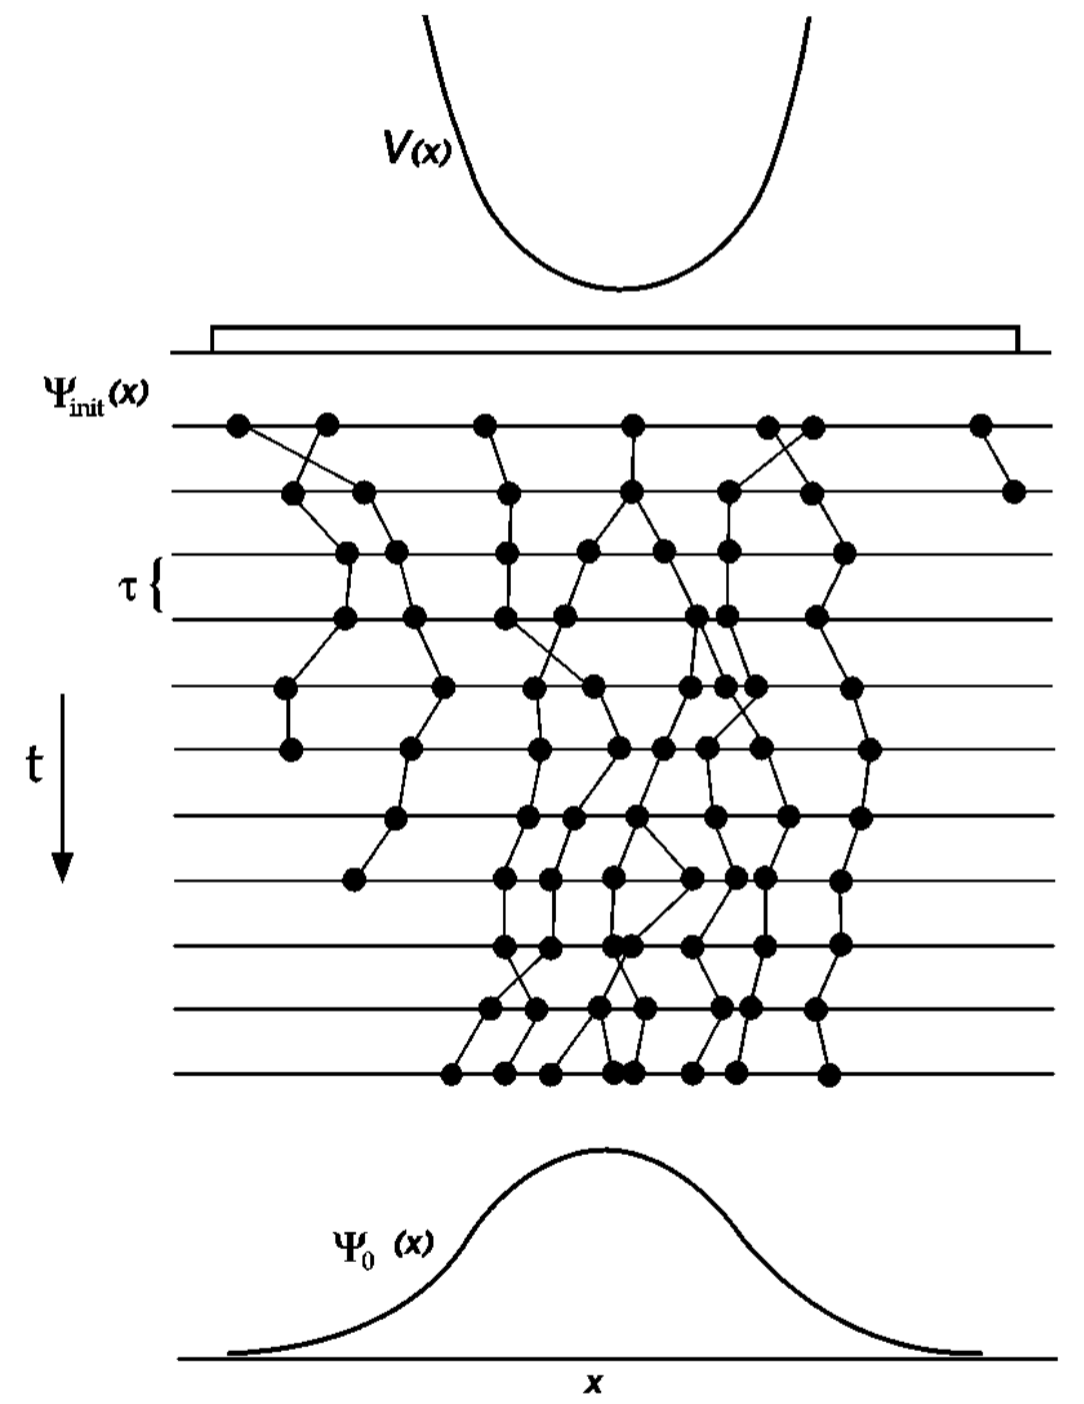
\includegraphics[width=0.4\textwidth]{figures/branching.png}
   \caption{Diagram describing the branching algorithm for Diffusion Monte Carlo (DMC). In this 1D example a particle is confined by the potential $V(x)$ and the trial wave function $\Psi_\text{init}(x)$ is propagated until it converges to the ground state wave function $\Psi_0(x)$. This diagram is from \cite{foulkes2001}.}
   \label{fig:branching}
\end{figure}

This sampling can have large uncertainties due to possible divergences in the branching weight in equation~\ref{equ:branchweight} as a result of particles getting too close or even coinciding. With the use of an importance function, $\Psi_I(\R)$ these fluctuations can be controlled without effecting the energy result. The importance function is used to bias the walker distributions toward $f(\R,t) = \Psi_T(\R,t)\Psi_I(\R)$ instead of $\Psi_T(\R,t)$ which effectively keeps the walkers away from locations where $\left|\Psi_T(\R,t)\right|^2$ is small.

This can be seen by multiplying Equation~\ref{equ:diffusion} by $\Psi_I(\R)$ and rewriting it in terms of $f(\R)$ as
\begin{equation}
   -\frac{1}{2}\nabla^2 f(\R,t) + \nabla\cdot\left[\mathbf{v}_D(\R) f(\R,t)\right] + \left[E_L(\R)-E_0\right]f(\R,t) = -\frac{\partial}{\partial t} f(\R,t),
\end{equation}
where $\mathbf{v}_D(R)$ is the drift velocity, defined as
\begin{equation}
   \mathbf{v}_D(\R) = \Psi_I(\R)^{-1}\nabla\Psi_I(\R) = \nabla \text{ln}\left|\Psi_I(\R)\right|.
\end{equation}
The drift velocity is responsible for pushing walkers away from areas of low $\left|\Psi_T(\R,t)\right|^2$. In practice the importance function is accounted for by directly sampling from
\begin{equation}
   G(\R',\R,\Delta\tau)\frac{\braket{\R}{\Psi_I}}{\braket{\R'}{\Psi_I}}
\end{equation}
instead of from the Green's function.

It is difficult to operate through the Green's function and so often observables are computed via mixed expectation values.
\begin{equation}
   \left<\mathcal{O(\tau)}\right>\text{mixed} = \frac{\bra{\Psi(\tau)}\mathcal{O}\ket{\Psi_T}}{\braket{\Psi(\tau)}{\Psi_T}}
\end{equation}
The true operator expectation value can approximately be written in terms of mixed expectation values \cite{pudliner1997} as
\begin{equation}
   \left<\mathcal{O(\tau)}\right> \approx 2\left<\mathcal{O(\tau)}\right>_\text{mixed} - \left<\mathcal{O}\right>_T,
   \label{equ:mixedexp}
\end{equation}
where
\begin{equation}
   \left<\mathcal{O}\right>_T = \frac{\bra{\Psi_T}\mathcal{O}\ket{\Psi_T}}{\braket{\Psi_T}{\Psi_T}}
\end{equation}
is the variational expectation value. Equation~\ref{equ:mixedexp} comes from a linear extrapolation of the mixed expectation value. For the Hamiltonian and operators that commute with the Hamiltonian the mixed expectation value is exactly the true expectation value for large time step. This can be seen directly with the Hamiltonian by splitting the Green's function up, to be used on either side of the Hamiltonian.
\begin{equation}
   \lim\limits_{\tau\rightarrow\infty}\left<H\right>_\text{mixed} = \frac{\bra{\Psi_T}e^{-H\tau/2}He^{-H\tau/2}\ket{\Psi_T}}{\bra{\Psi_T}e^{-H\tau/2}e^{-H\tau/2}\ket{\Psi_T}} = E_0
\end{equation}

The nuclear wave function is antisymmetric and will change sign as particle interact and exchange. As a result the oscillatory nature of the wave function requires positive and negative terms to cancel in the integral. Very accurate calculations must be done to accurately calculate these cancellations, and as a result very large uncertainties can be obtained. One approximate solution to this is the fixed-node approximation \cite{moskowitz1982}. The basic idea is that the trial wave function defines a nodal surface that is zero at the surface and changes sign across the surface. The wave functions are not allowed to cross the nodal surface. This maintains the upper bound principle of VMC, and is exact if the trial wave function, from which the nodal surface is defined, is exactly the ground state. This method assumes that the wave function is real, which is usually not the case with spin-isospin interactions. A generalization called the constrained path method works for real and complex wave functions alike \cite{wiringa2000}. The general idea is that walker configurations that have negative or zero overlap with the propagated wave function are discarded. This is only an approximate approach that depends on the choice of $\Psi_T(\R)$ and does not guarantee an upper bound on the energy. To this day there is active research looking for efficient ways to solve the Fermi-sign problem in many-body quantum systems. In practice we follow the method used in \cite{zhang2003} by using the real part of the trial wave function as the importance function and setting the weight to zero for any configuration whose overlap with the propagated wave function is zero or negative. This guarantees that the weights will be real and positive.

The constraint gives a non-exact result, however better convergence to the exact answer can be obtained by generating a set of good configurations with the constraint and then releasing the constraint for typically 20 to 40 steps to calculate the energy. Small systems, $A\le4$, will often converge before the statistical error overwhelms the signal. For larger systems an exponential extrapolation is typically used to determine the final energy as in \cite{pudliner1997}.

The DMC algorithm can generally be written as follows.
\begin{enumerate}
   \item Generate a set of random walkers. These are typically from the results of a VMC calculation, which has no constraint and provides an upper bound in the energy.
   \item For each walker propose a move, $\R' = \R + \mathbf{\chi}$, where $\mathbf{\chi}$ is a vector of random numbers from the shifted Gaussian $\exp\left(\frac{m}{2\hbar^2\Delta\tau}\left(\R'-\R+2\frac{\nabla\Psi_I(\R')}{\Psi_I(\R')}\right)^2\right)$.
   \item For each walker calculate the weight $w(\R')=\exp\left(-\left(\frac{E_L(\R')+E_L(\R)}{2}-E_0\right)\Delta\tau\right)$.
   \item Do branching.
   \item Calculate and collect the observables and uncertainties needed and increase the imaginary time by $\Delta\tau$.
   \item Repeat steps 2 through 5 until the uncertainties are small enough.
\end{enumerate}

The uncertainties are calculated by block averaging. The data we generate is inherently autocorrelated because each step in the Markov chain depends on the last. This will underestimate the statistical error in our calculation. The idea of block averaging is to form blocks in our data such that the average over each block is not correlated with the last block. This gives us a good estimate for the statistical uncertainty. In practice the block size is chosen so that the error estimate will not increase as the block size is increased. This is illustrated in the sample data shown in Figure~\ref{fig:blockaverage}.
\begin{figure}[h!]
   \centering
   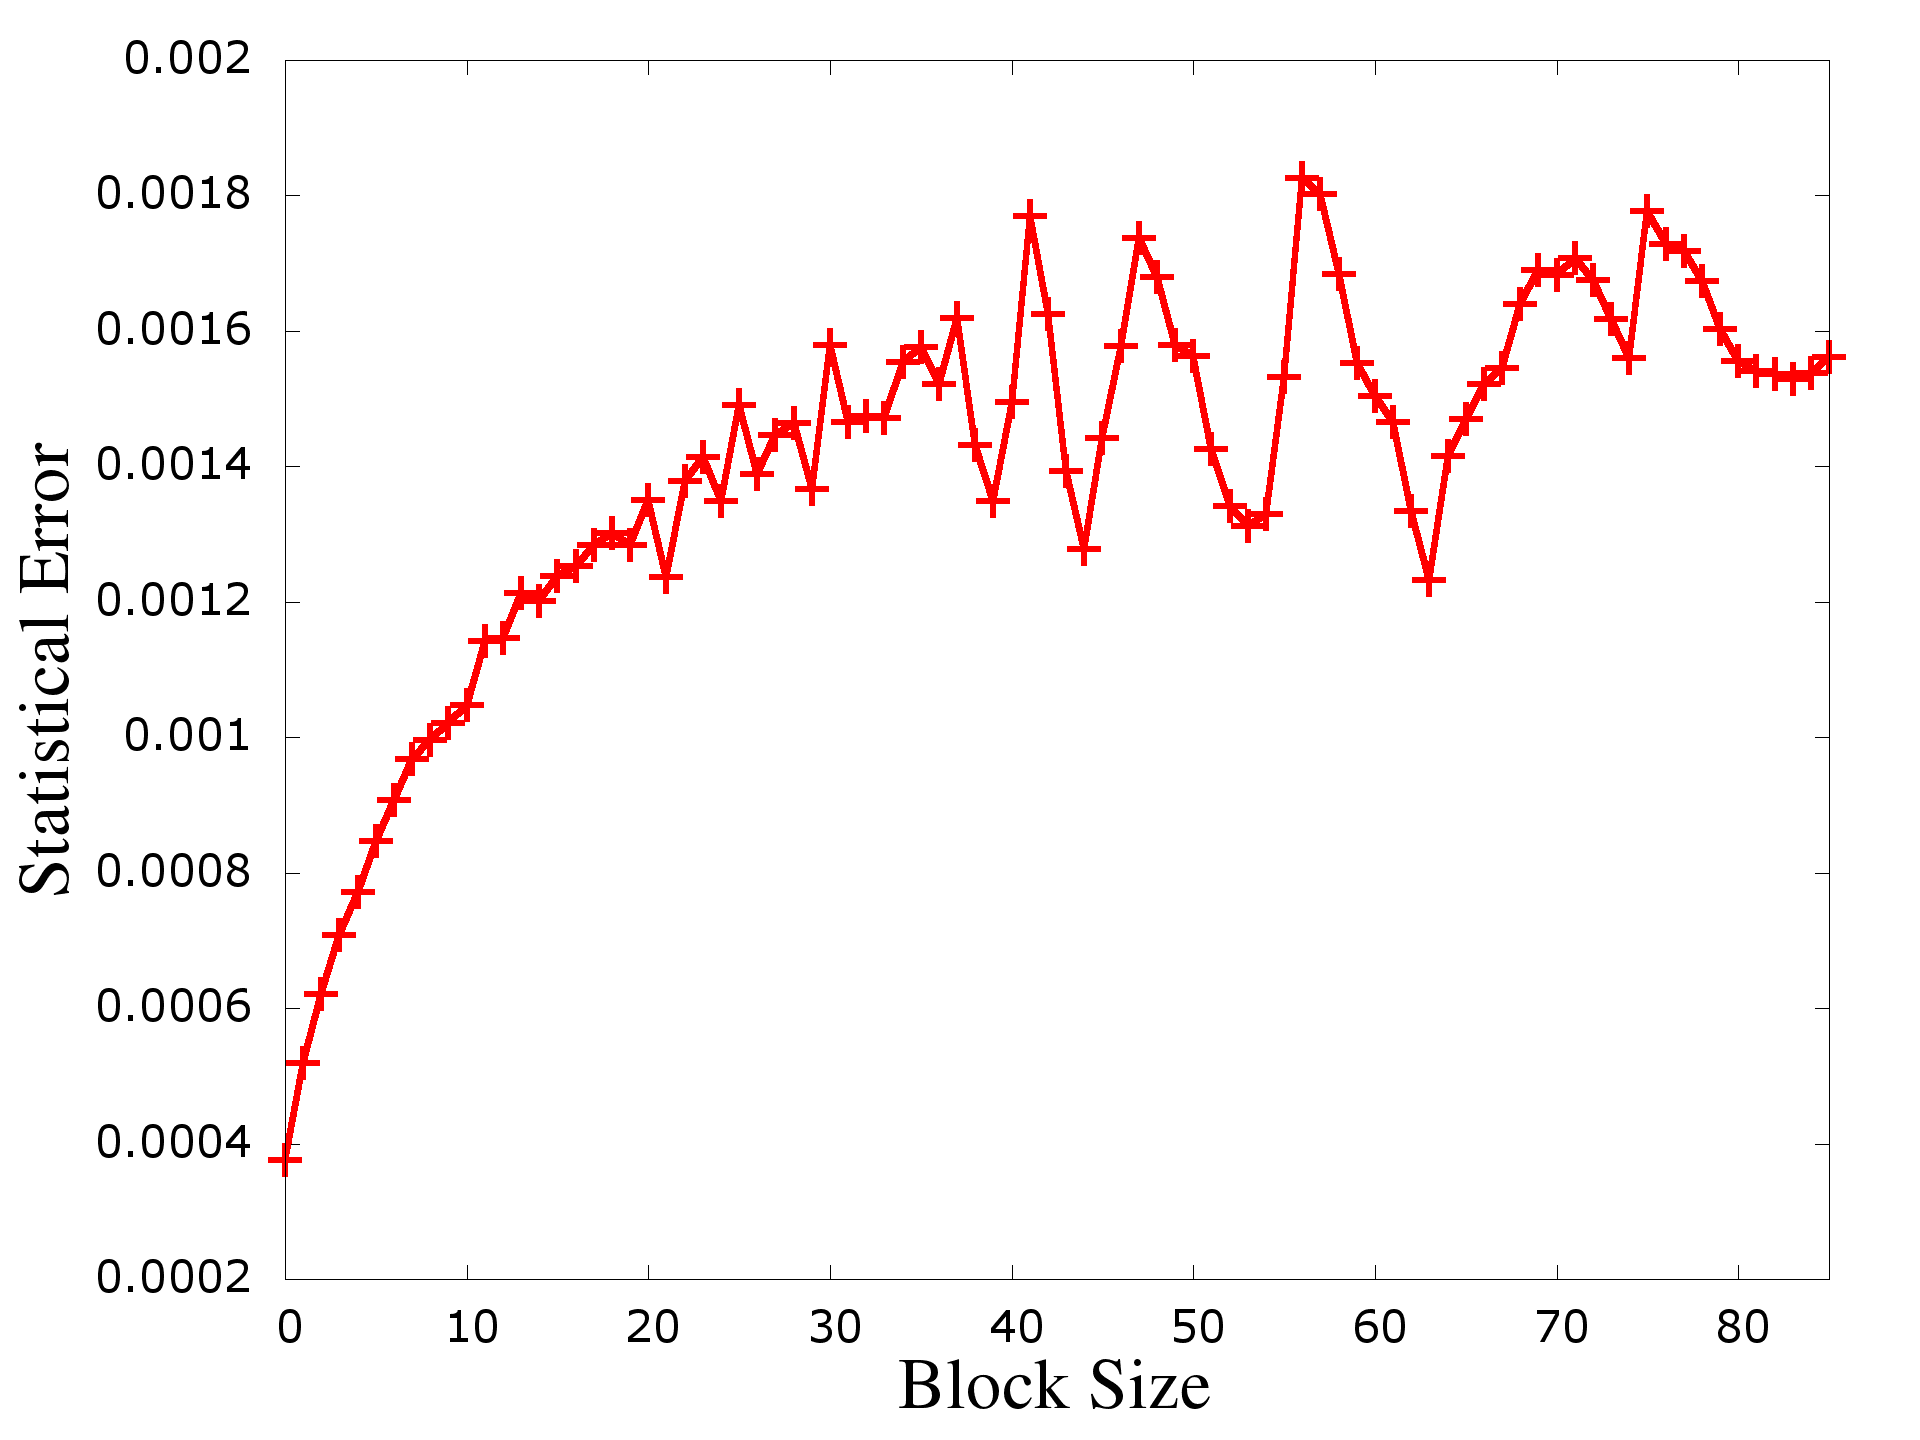
\includegraphics[width=0.7\textwidth]{figures/blockaverage.png}
   \caption{Sample data showing the convergence of the statistical uncertainty as the block size is increased. An appropriate block size for this data would be about 35, where the errors stop increasing with block size.}
   \label{fig:blockaverage}
\end{figure}

Good reviews of this method can be found in Refs. \cite{foulkes2001} and  \cite{carlson2015}. DMC only accounts for spin-isospin independent Hamiltonians, unlike Green's function Monte Carlo (GFMC) and auxiliary field diffusion Monte Carlo (AFDMC) which follow DMC for sampling spatial states but use two different methods to sample spin-isospin states. For each set of spatial integrals there is a sum over all of the spin and isospin states. GFMC evaluates this sum explicitly. This is inefficient as the number of spin states scales as
\begin{equation}
   \frac{A!}{Z!(A-Z)!}2^A
\end{equation}
where $A$ is the number of nucleons and $Z$ is the number of protons.
%The number of possible spin states given $A$ nucleons is $2^A$. The number of isospin states given $A$ nucleons and $Z$ protons can be reduced to ${A \choose Z}$ states leaving us with a total of $2^A {A \choose Z}$ spin-isospin states.
The number of states and the number of operators required for the trial wave function increase exponentially as the number of nucleons increases. To date, the largest nuclei that can be calculated with GFMC is ${}^{12}C$ \cite{lovato2013,lovato2014,lovato2015}. AFDMC was developed as an alternative to the explicit sum over spin-isospin states that GFMC performs.

\subsection{Auxiliary Field Diffusion Monte Carlo}
\label{sec:AFDMC}
To overcome the exponentially large number of spin-isospin states that have to be summed in GFMC, AFDMC was developed in 1999 \cite{schmidt1999} to sample spin and isospin states and, in analogy to moving the position of each walker, rotate the spin and isospin of each walker. The walkers are defined by the three spatial positions and amplitude for each particle to be in each of the four possible spin-isospin states $\ket{s} = \ket{p\uparrow,p\downarrow,n\uparrow,n\downarrow}$. The Hamiltonian can then be broken up into spin-isospin independent $H_{SI}$ and spin-isospin dependent $H_{SD}$ parts. The spin-isospin dependent part only comes from the potential and can be written as $V_{SD}$. The propagator can be broken up to have the old propagator used in DMC, which is independent of spin and isospin, and a spin-isospin dependent piece.
\begin{equation}
   G(\R'S',\R S,\tau)=\bra{\R'}e^{-(H-E_0)\tau}\ket{\R}G_{SD}(\R'S',\R S,\tau)
\end{equation}
where the spin-isospin dependent part of the propagator is
\begin{equation}
   G_{SD}(\R'S',\R S,\dt) = \bra {\R'S'}e^{-V_{SD}\dt} \ket{\R S}.
\end{equation}
The spin-isospin dependent part of the potential can be written as
\begin{equation}
   V_{SD} = \sum\limits_{p=2}^{M}\sum\limits_{i<j} \vpij\Opij,
\end{equation}
where M is the number of operators (e.g. $M=6$ for the AV6$'$ potential or $M=18$ for the Argonne AV18 two-body potential \cite{wiringa1984}). In this study I have used the standard AV6$'$ potential which includes the operators $\si\cdot\sj$, $\ti\cdot\tj$, $\si\cdot\sj \ti\cdot\tj$, $S_{ij}$ and $S_{ij} \ti\cdot\tj$, where $S_{ij} = 3\si\cdot\hat{r}_{ij}\sj\cdot\hat{r}_{ij}-\si\cdot\sj$. Here the $\mathbf{\si}$ and $\mathbf{\ti}$ operators are the Pauli matrices applied to spin and isospin of the $i$-th particle respectively.

AFDMC samples the spin and isospin states by expressing the operators in terms of squared single-particle particle operators which are transformed via the Hubbard-Stratanovich transformation. This can be done if the operators are expressed in the more convenient form
\begin{equation}
   V_{SD} = \frac{1}{2}\sum\limits_{i,\alpha,j,\beta} \sigma_{i,\alpha}A^{\sigma}_{i,\alpha,j,\beta}\sigma_{j,\beta}
      + \frac{1}{2}\sum\limits_{i,\alpha,j,\beta} \sigma_{i,\alpha}A^{\sigma\tau}_{i,\alpha,j,\beta}\sigma_{j,\beta}\ti\cdot\tj
      + \frac{1}{2}\sum\limits_{i,j} A^{\tau}_{i,j}\ti\cdot\tj,
   \label{equ:VwithA}
\end{equation}
where we have defined new $A$ matrices. The $A$ matrices are written in terms of the $\vpij$ functions above. For example the simplest matrix is the $A^{\tau}_{i,j}$ matrix which can be shown to be $A^{\tau}_{i,j} = v_{\tau}(r_{ij})$. There is a factor of one half in Eq.~\ref{equ:VwithA} because the sums go over all $i$ and $j$ particles instead of pairs for which $i<j$. These matrices are zero when $i=j$ and they are symmetric. We can also write these matrices in terms of their eigenvalues and eigenvectors.
\begin{align}
   &\sum\limits_{j,\beta} A^{\sigma}_{i,\alpha,j,\beta}\psi^{\sigma}_{n,j,\beta} = \lambda^{\sigma}_n\psi^{\sigma}_{n,i,\alpha} \\
   &\sum\limits_{j,\beta} A^{\sigma\tau}_{i,\alpha,j,\beta}\psi^{\sigma\tau}_{n,j,\beta} = \lambda^{\sigma\tau}_n\psi^{\sigma\tau}_{n,i,\alpha} \\
   &\sum\limits_{j} A^{\tau}_{i,j}\psi^{\tau}_{n,j} = \lambda^{\tau}_n\psi^{\tau}_{n,i}
\end{align}
Written in terms of these eigenvalues and eigenvectors the potential can be written as
\begin{equation}
   V_{SD} = \frac{1}{2}\sum\limits_{n=1}^{3A} \left(O_{n}^{\sigma}\right)^2 \lambda_n^{\sigma}
      + \frac{1}{2}\sum\limits_{\alpha=1}^{3}\sum\limits_{n=1}^{3A} \left(O_{n\alpha}^{\sigma\tau}\right)^2 \lambda_n^{\sigma\tau}
      + \frac{1}{2}\sum\limits_{\alpha=1}^{3}\sum\limits_{n=1}^{A} \left(O_{n\alpha}^{\tau}\right)^2 \lambda_n^{\tau},
\end{equation}
where the operators are given by
\begin{equation}
\begin{split}
   O_{n}^{\sigma} &= \sum\limits_{j,\beta} \sigma_{j,\beta}\psi_{n,j,\beta}^{\sigma} \\
   O_{n\alpha}^{\sigma\tau} &= \sum\limits_{j,\beta} \tau_{j,\alpha}\sigma_{j,\beta}\psi_{n,j,\beta}^{\sigma\tau} \\
   O_{n\alpha}^{\tau} &= \sum\limits_{j} \tau_{j,\alpha}\psi_{n,j}^{\tau}.
\end{split}
\end{equation}
These operators in the propagator now have the effect of rotating the spinors, analogous to diffusing the walkers in space. To reduce the order of the operators in the propagator from quadratic to linear we use the Hubbard-Stratanovich transformation.
\begin{equation}
   e^{-\frac{1}{2}\lambda O^2} = \frac{1}{\sqrt{2\pi}} \int dx e^{-\frac{x^2}{2} + \sqrt{-\lambda}x O}
\end{equation}
The variable $x$ is called an auxiliary field. Using the fact that there are $3A$ $O_{n}^{\sigma}$ operators, $9A$ $O_{n\alpha}^{\sigma\tau}$ operators and $3A$ $O_{n\alpha}^{\tau}$ operators, for a total of $15A$ operators, and by using the Hubbard-Stratanovich transformation we can write the spin-isospin dependent part of the propagator as
\begin{equation}
   G_{SD}(\R'S',\R S,\dt) = \bra{\R'S'}\prod\limits_{n=1}^{15A}\frac{1}{\sqrt{2\pi}}\int dx_n e^{-\frac{x_n^2}{2}}e^{\sqrt{-\lambda_n\dt} x_nO_n}\ket{\R S}.
   \label{equ:GSD}
\end{equation}
The spinors are rotated based on auxiliary fields sampled from the Gaussian with unit variance in Eq.~\ref{equ:GSD}. The sampling of the auxiliary fields is done in exactly the same way as the sampling of the spatial walkers in DMC, with the Markov chain Metropolis algorithm. Each sampled auxiliary field depends only on the previous sample and no more history than that.

Importance sampling can be included in the Auxiliary Field sampling in a similar way as described before with DMC. However, in practice it is done as follows. The $\Delta \R$ and $\Delta x_n$ are sampled by symmetric Gaussians and so the probability of $\Delta \R$ and $-\Delta \R$, and $\Delta x_n$ and $-\Delta x_n$ are the same. As a result the weight for the four possible combinations are sampled as
\begin{align}
   w_1 &= \frac{\braket{\Psi_I}{\R+\Delta \R, S'(x_n)}}{\braket{\Psi_I}{\R S}} e^{\left(-V_{SI}(\R+\Delta\R) - E_0\right)\dt} \\
   w_2 &= \frac{\braket{\Psi_I}{\R-\Delta \R, S'(x_n)}}{\braket{\Psi_I}{\R S}} e^{\left(-V_{SI}(\R-\Delta\R) - E_0\right)\dt} \\
   w_3 &= \frac{\braket{\Psi_I}{\R+\Delta \R, S'(-x_n)}}{\braket{\Psi_I}{\R S}} e^{\left(-V_{SI}(\R+\Delta\R) - E_0\right)\dt} \\
   w_4 &= \frac{\braket{\Psi_I}{\R-\Delta \R, S'(-x_n)}}{\braket{\Psi_I}{\R S}} e^{\left(-V_{SI}(\R-\Delta\R) - E_0\right)\dt},
\end{align}
and the sample with the largest weight is used. The weight for the chosen configuration, which is used for branching, is the average of the four weights
\begin{equation}
   W = \frac{1}{4}\sum\limits_{n=1}^4 w_n.
\end{equation}

\subsection{Hamiltonian}
One of the difficulties in many-body nuclear physics is finding an accurate Hamiltonian that is easy to calculate with the method you have selected. For QMC methods the Hamiltonian must be in configuration space and it must be local. Small degrees of non-locality can be addressed \cite{lynn2012,lynn2013}. Also, the nuclear physics Hamiltonian must be able to account for 2-body and 3-body interactions. The most generic form for the nuclear Hamiltonian then takes the form
\begin{equation}
   H = -\frac{\hbar^2}{2m}\sum\limits_i \nabla_i^2 + \sum\limits_{i<j} v_{ij} + \sum\limits_{i<j<k} V_{ijk} + \ldots.
\end{equation}
In principle there could be higher order terms included the in practice the two-nucleon NN interaction $v_{ij}$ and the three-nucleon interaction (TNI) $V_{ijk}$ are the only terms included as the importance of an $n$-nuclear potential decreases as $n$ increases. Calculations with only NN potentials will often underbind nuclei with $A>2$ and it has been shown that the inclusion of the TNI interaction improves this underbinding as well as level ordering in the excitation spectra of nuclei. This improvement has been shown in GFMC \cite{fantoni2008} as well as other methods such as the no-core shell model \cite{navratil2003}.

The NN potential takes the form
\begin{equation}
   v_{ij} = \sum\limits_{p=1}^M v_p(\r_{ij})\mathcal{O}^p_{ij},
\end{equation}
where $M$ is the number of operators begin used.
Two-nucleon potentials are often fit to NN scattering data and several very accurate models have been developed including the Nijmengen \cite{nagels1975,stoks1994}, CD-Bonn \cite{machleidt1996,machleidt2001}, and Argonne $v$18 (AV18) potentials \cite{wiringa1984,wiringa1995}. The Argonne potential is one of the most accurate and will be used in this work. The AV18 potential has 18 operators coming from one- and two-pion exchange as well as phenomenological sources. Often a subset of the AV18 potential is used, e.g. AV4$'$, AV6$'$, AV8$'$ or AV14$'$. These AV$n'$ potentials have kept only the top $n$ most important terms and are refit to scattering data at that level. A study of the successive importance of these terms up to $n=8$ compared with the full AV18 with and without three-nucleon potentials is given in \cite{wiringa2002}. The operators of the AV18 potential are
\begin{align}
   \mathcal{O}_{ij}^{p=1,8} &= \left[1,\si\cdot\sj,S_{ij},\mathbf{L}\cdot\mathbf{S}\right]\otimes\left[1,\ti\cdot\tj\right], \\
   \mathcal{O}_{ij}^{p=9,14} &= \left[\mathbf{L}^2,\mathbf{L}^2\si\cdot\sj,(\mathbf{L}\cdot\mathbf{S})^2\right]\otimes\left[1,\ti\cdot\tj\right], \\
   \mathcal{O}_{ij}^{p=15,18} &= \left[T_{ij},\si\cdot\sj T_{ij},S_{ij}T_{ij},\tau_i^2+\tau_j^2\right],
\end{align}
where the tensor term is $S_{ij} = 3\si\cdot\hat{r}_{ij}\sj\cdot\hat{r}_{ij}-\si\cdot\sj$, the $\mathbf{L}\cdot\mathbf{S}$ term is the spin-orbit term, and the $T_{ij} = 3\tau_i^2\tau_j^2-\ti\cdot\tj$ is the isotensor term.

In this work the AV6$'$ potential is used, which includes all of the same operators as AV8$'$ except for those including the spin-orbit terms, $\left[1,\si\cdot\sj,S_{ij}\right]\otimes\left[1,\ti\cdot\tj\right]$. The functions multiplying the AV6$'$ operators are shown in figure \ref{fig:vij}.
\begin{figure}[h!]
   \centering
   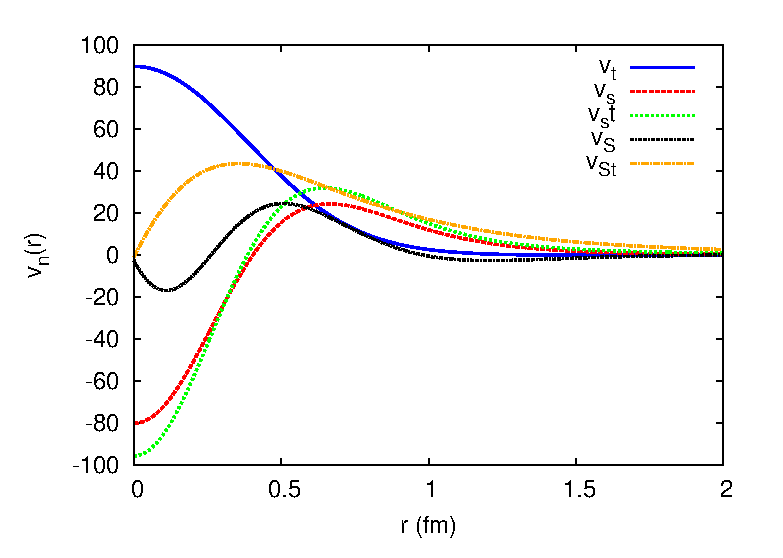
\includegraphics[width=0.7\textwidth]{figures/vij.eps}
   \caption{The functions multiplying the AV6$'$ operators as a function of nucleon separation. The central operator is excluded to show the spin-isospin terms with better detail. The $v_s$ represents the spin operators, $v_t$ the isospin operators, $v_{st}$ the spin-isospin operators, $v_S$ the tensor, and $v_{St}$ the tensor-isospin operators.}
   \label{fig:vij}
\end{figure}

The AV6$'$ can be broken up in Cartesian coordinates including 39 operators, 3 from $\tau$, 9 from $\sigma$, and 27 from $\sigma\tau$ terms. This can be done by writing the potential in the form
\begin{equation}
   \sum\limits_p v_p(\r_{ij})\mathcal{O}^p_{ij} = v_1(\r_{ij}) + \sum\limits_\alpha \t_{i\alpha}A^\tau_{ij}\t_{j\alpha} + \sum\limits_{\alpha,\beta} \s_{i\alpha}A^\sigma_{ij}\s_{j\beta} + \sum\limits_{\alpha,\beta,\gamma} \s_{i\alpha}\t_{i\gamma}A^{\sigma\tau}_{ij}\s_{j\beta}\t_{j\gamma},
\end{equation}
where the matrices are given by
\begin{align}
   A^\tau_{ij} &= v_2(\r_{ij}), \\
   A^\sigma_{ij} &= v_3(\r_{ij})\delta_{\alpha\beta} + v_5(\r_{ij})(3\rij^\alpha\rij^\beta-\delta_{\alpha\beta}), \\
   A^{\sigma\tau}_{ij} &= v_5(\r_{ij})\delta_{\alpha\beta} + v_6(\r_{ij})(3\rij^\alpha\rij^\beta-\delta_{\alpha\beta}).
\end{align}
This is a simple way to break up the AV6$'$ potential but a more efficient breakup can be used in which only 15 operators are needed. This is achieved by using $\rij$ as the first basis function and then using two additional orthogonal basis functions. This reduces the $\rij^\alpha\rij^\beta$ term in the matrices to $\delta_{\alpha\beta}$. This potential can then be written as
\begin{equation}
   \sum\limits_p v_p(\r_{ij})\mathcal{O}^p_{ij} = v_1(\r_{ij}) + \sum\limits_\alpha \t_{i\alpha}A^\tau_{ij}\t_{j\alpha} + \sum\limits_{\alpha} \s_{i\alpha}A^\sigma_{ij}\s_{j\alpha} + \sum\limits_{\alpha,\gamma} \s_{i\alpha}\t_{i\gamma}A^{\sigma\tau}_{ij}\s_{j\alpha}\t_{j\gamma},
\end{equation}
where the matrices are given by
\begin{align}
   A^\tau_{ij} &= v_2(\r_{ij}), \\
   A^\sigma_{ij} &= v_3(\r_{ij}) + 2v_5(\r_{ij}), \\
   A^{\sigma\tau}_{ij} &= v_5(\r_{ij}) + 2v_6(\r_{ij}),
\end{align}
where it is easy to see that there are 3 $\tau$, 3 $\sigma$, and 9 $\sigma\tau$ terms for a total of 15 operators in this basis.

Calculations with $A\le2$ are well described by the NN potentials, however for any system with $A\ge3$ the 3-nucleon force is needed to accurately describe the system. The phenomenological 3-nucleon forces that are typically employed in AFDMC calculations are the older Urbana and newer Illinois potentials. The Urbana IX (UIX) potential is built using the two-pion three-nucleon interaction, which can be written as
\begin{equation}
\begin{split}
   V_{2\pi3N} = \sum\limits_\text{cycl.} &A_{2\pi}\{\t_1\cdot\t_2,\t_1\cdot\t_3\} \{(S_{12}T(\r_{12})+\s_1\cdot\s_2 Y(\r_{12})),(S_{13}T(\r_{13})+\s_1\cdot\s_3 Y(\r_{13}))\} \\
      + &C_{2\pi}\left[\t_1\cdot\t_2,\t_1\cdot\t_3\right] \left[(S_{12}T(\r_{12})+\s_1\cdot\s_2 Y(\r_{12})),(S_{13}T(\r_{13})+\s_1\cdot\s_3 Y(\r_{13}))\right] \\
      + &B(\r_{12},\r_{13})\{\t_1\cdot\r_2,\t_1\cdot\t_3\}\{(S_{12}+\s_1\cdot\s_2),(S_{13}+\s_1\cdot\s_3)\},
\end{split}
\end{equation}
where the sum is a cyclic sum over 1, 2, and 3. The $\{~,~\}$ and $[~,~]$ are anticommutators and commutators and the $Y(r)$ and $Y(r)$ are the radial Yukawa and one-pion exchange interactions as described in \cite{carlson1983},
\begin{align}
   Y(r) &= \frac{e^{-\mu r}}{\mu r} Y_\text{cut}(r) \\
   T(r) &= \left(1+\frac{3}{\mu r} + \frac{3}{\mu^2 r^2}\right)\frac{e^{-\mu r}}{\mu r} T_\text{cut}(r),
\end{align}
where $Y_\text{cut}(r)$ and $T_\text{cut}(r)$ are the cutoff functions for the Yukawa and one-pion exchange terms respectively. The $B(\r_{12},\r_{13})$ term comes from $\pi$N s-wave scattering. The UIX potential is fit to the ground states of $^3$H and $^4$He. For details about the construction and results obtained with this potential I refer the reader to \cite{carlson1983, pudliner1996, pudliner1997}.

The Illinois-7 (IL7) potential \cite{pieper2001} contains two-pion three-nucleon interactions in both the s-wave and p-wave, as well as a three-pion exchange and three-nucleon contact interactions. The IL7 potential has been fit to the low-lying spectra of nuclei with $A=3$ to nuclei with $A=10$. These phenomenological potentials have been used to calculate many properties of light nuclei with high accuracy using both the GFMC and AFDMC methods.

Despite the accuracy of these potentials they have little direct connection to the underlying theory of QCD. In recent years a set of nuclear potentials has been developed from a chiral effective field theory ($\chi$EFT) framework that can be used with nuclear QMC methods such as GFMC and AFDMC \cite{epelbaum2009,machleidt2011}. These potentials are local up the next-to-next-to leading order (N$^2$LO) and so QMC calculations can use potentials up to this order. Good results using these potentials have been obtained with both GFMC \cite{lynn2014} and AFDMC \cite{lonardoni2018}.

All calculations here have been done with the AV6$'$ potential to reduce computation requirements as well as to better focus on the improvements made by improved wave functions. It would be straightforward to do any of these calculations with the three-nucleon and the $\chi$EFT potentials.

\chapter{Trial Wave Function}
An accurate trial wave function can drastically improve the accuracy of a variational QMC method such as VMC and AFDMC. Most highly accurate trial wave functions are computationally intractable and are never implemented in QMC methods. In addition to being accurate and computationally tractable a good wave function must satisfy known physical properties such as cluster decomposition as well as having an overall antisymmetry with respect to particle exchange due to the spin-1/2 property of nucleons.

Cluster decomposition arises from the physical intuition that the wave function of two separate, non-interacting systems, $A$ and $B$ as in Figure~\ref{fig:cluster}, can be written as the outer product of their respective wave functions.
\begin{figure}[h]
   \centering
   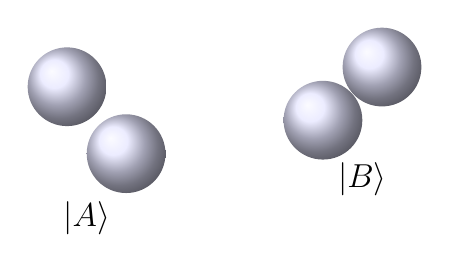
\begin{tikzpicture}[>=latex,scale=0.5]
      \shade[ball color=blue!10!] (-4.0,0.85) circle (1) ;
      \shade[ball color=blue!10!] (-2.5,-0.85) circle (1) ;
      \shade[ball color=blue!10!] (4.0,1.35) circle (1) ;
      \shade[ball color=blue!10!] (2.5,0.00) circle (1) ;
      \draw (-3.5,-2.5) node{\large $\ket{A}$};
      \draw (3.5,-1.5) node{\large $\ket{B}$};
   \end{tikzpicture}
   \caption{Two non interacting systems $A$ and $B$, whose composite wave function is the product $\ket{A+B}=\ket{A}\ket{B}$.}
   \label{fig:cluster}
\end{figure}
If a system is not cluster decomposable, nonphysical correlations between non-interacting systems can occur.

The second property is that the wave function be antisymmetric overall. Since nucleons are fermions and the only degrees of freedom used in these calculations the product of different pieces of the wave function must be antisymmetric. Recent work in QMC has successfully included bosonic degrees of freedom such as pions (\cite{madeira2018}), however that is not the case in this work.

%\begin{figure}[h!]
%   \centering
%   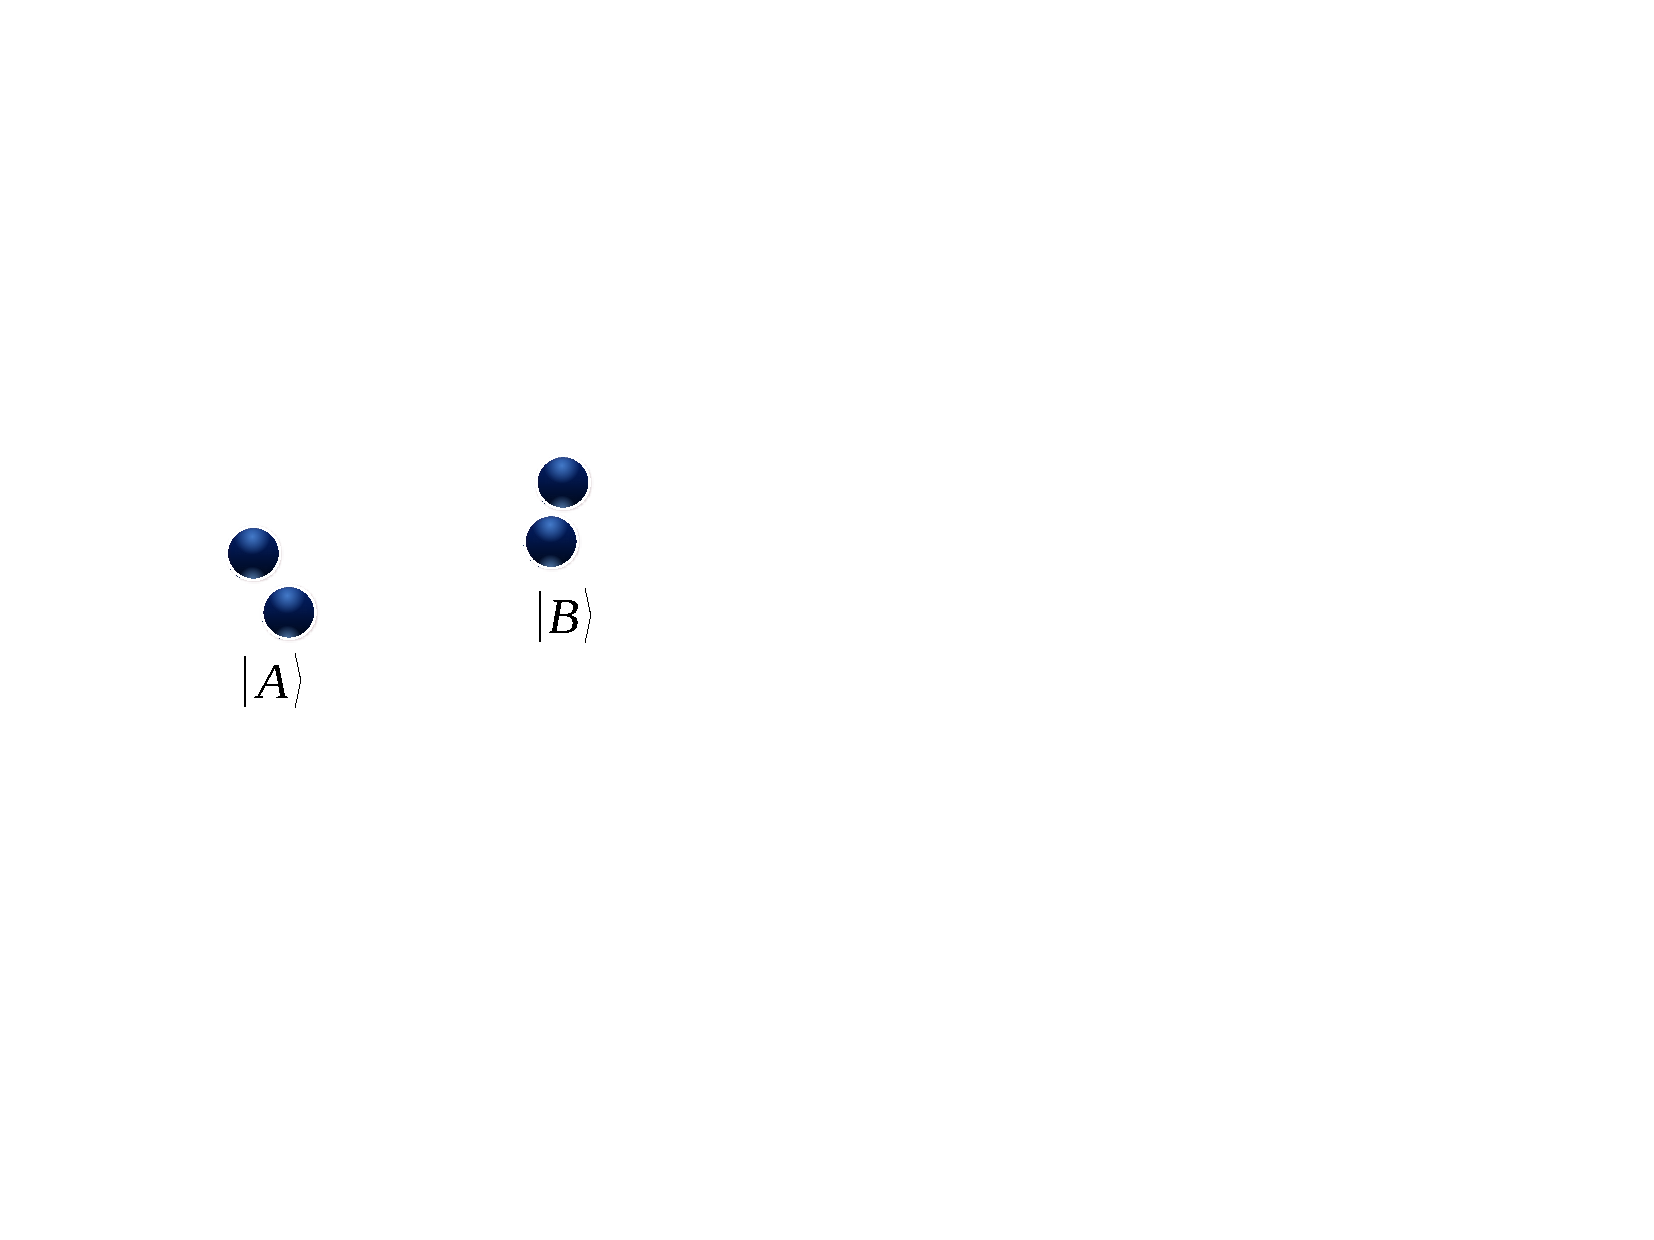
\includegraphics[width=\textwidth]{figures/cluster.pdf}
%   \caption{Energy per nucleon for ${}^4$He and ${}^{16}$O as calculated with linear, independent pair and quadratic correlations. Also, the energy per nucleon of symmetric nuclear matter of 28 particles in a periodic box with density $\rho=0.16$fm$^{-3}$. All calculations are compared to their expected values.}
%   \label{fig:cluster}
%\end{figure}

\section{Slater Determinant}
One of the simplest wave functions that satisfies the two properties specified above is the Slater determinant. The Slater determinant has been the starting place for a variety of many-body calculations in nuclear and condensed matter physics alike. In condensed matter the many-body wave functions will often be written in terms of a sum of weighted Slater determinants, where some methods have been able to use a sum of up to 2 billion determinants (\cite{huron1973,li2018}). In nuclear physics a single determinant is often used for closed shell calculations and a sum of a small number  of weighted determinants is used for open shell systems. For small to medium mass open-shell nuclei on the order of 10 or 100 determinants are often used. A Slater determinant is an antisymmetrized product of single particle, non-interacting, wave functions
\begin{equation}
   \Psi_{SD}(\R,S) = \mathcal{A} \left[\phi_1(\r_1)\phi_2(\r_2) \ldots \phi_A(\r_A)\right] =
   \begin{vmatrix}
      \phi_1(\r_1) & \phi_1(\r_2) & \ldots & \phi_1(\r_A) \\
      \phi_2(\r_1) & \phi_2(\r_2) & \ldots & \phi_2(\r_A) \\
      \vdots & \vdots & \ddots & \vdots \\
      \phi_K(\r_1) & \phi_K(\r_2) & \ldots & \phi_K(\r_A) \\
   \end{vmatrix},
\end{equation}
where $\R$ and $S$ are the spatial and spin coordinates of the walkers, $\mathcal{A}$ is the antisymmetrization operator, and the $\phi_i(\r_j)$ are the overlap of the walker positions with the model single particle states, $\braket{\r_j}{\phi_i}$. The single particle model states are made up of a radial and spin, iso-spin dependent parts,
\begin{equation}
   \phi_k = \Phi_{nj}\left[C_{c_l,m_s}^j Y_{l,m_l}(\hat{r}_i)\chi_s(s_i)\right]_{j,m_j},
\end{equation}
where $\Phi_{nj}$ is the radial part and the rest contains the spherical harmonics $Y_{l,m_l}(\hat{r}_I)$ and spin and iso-spin states where the Clebsch-Gordan coefficients ensure the correct $j$ and $m_j$ quantum numbers, and the different states are given by the index $k$. To accurately describe the wave function of an open shell nuclei each state with the correct total angular momentum, parity $J^\pi$, and isospin $T$ is included as a separate Slater determinant.
\begin{equation}
   \braket{\R S}{\Phi}_{J^\pi,T} = \sum\limits_n c_n D\{\phi_k(\r_i,s_i)\}
\end{equation}
Here the $c_n$ coefficients are variational parameters used to minimize the energy given a set of possible state configurations. One of the simplest examples of an open shell nuclei would be $^6$He whose ground state is a $J^\pi = 0^+$ state. The two protons and two of the neutrons could be in the full $(1S_{1/2})^2$ shell while the two remaining neutrons could be in the $(1P_{3/2})^2$ shell with their $m_j=\pm 3/2, \pm 1/2$ values being equal and opposite to ensure that $J=0$. This state has two possible determinants. Other possible configurations for the two remaining neutrons would be $(1P_{1/2})^2$ with one possible determinant, $(1D_{5/2})^2$ with three possible determinants, $(2S_{1/2})^2$ with one possible determinant and $(1D_{3/2})^2$ with two possible determinants giving a total of nine possible determinants. Notice that the two neutrons could be in a combination of $S$ and $D$ shells but never an $S$ and $P$ or $D$ and $P$ to ensure the parity of the state is positive. The number of determinants used for open shell nuclei will control how accurate the trial wave function is. For closed shell nuclei such as $^4$He or $^{16}$O a single Slater determinant describing the full shell configuration is sufficient.

The radial part $\Phi_{nj}$ of the single particle states are obtained as bound state solutions to the single particle Schr\"odinger equation with a Woods-Saxon potential wine-bottle potential.
\begin{equation}
   v(r) = V_s\left[\frac{1}{1+e^{(r-r_s)/a_s}} + \alpha_se^{(-r/\rho_s)^2}\right]
\end{equation}
Here the parameters, $V_s, r_s, a_s, \alpha_s$ and $\rho_s$ are variational parameters used to shape the potential to obtain a minimum in energy.

%As an illustrative example consider the deuteron. The deuteron is in a iso-spin singlet state, $\frac{1}{\sqrt{2\pi}}(\ket{pn}-\ket{np})$. To show how the model state, $\ket{\Phi}$ would be built for this I will assume all entries are 1, though in practice the could all take on different numbers to account for the different spacial and spin dependencies of the state. Let's assume that both the neutron and the proton are in a spin up state. In this case the $\Phi(k,i)$ terms, where $k,i=1,2$, would take on the following values.
%\begin{align}
%   \phi(1,1)&=(1,0,0,0)=p\uparrow_1 \\
%   \phi(2,1)&=(0,0,1,0)=n\uparrow_1 \\
%   \phi(1,2)&=(1,0,0,0)=p\uparrow_2 \\
%   \phi(2,2)&=(0,0,1,0)=n\uparrow_2
%\end{align}
%The determinant of the Slater matrix can then be written as
%\begin{equation}
%\Psi_T=\det(S)=
%\begin{vmatrix}
%    \braket{k_1}{s_1} & \braket{k_1}{s_2} \\
%    \braket{k_2}{s_1} & \braket{k_2}{s_2}
%\end{vmatrix}
%=
%\begin{vmatrix}
%    p_1 & p_2 \\
%    n_1 & n_2
%\end{vmatrix}
%=
%p_1n_2-n_1p_2,
%\end{equation}
%which is the singlet state that we wanted to start with.

The Slater determinant is a mean-field wave function and is often used with Jastrow type short range correlations.
\begin{equation}
   \braket{\R S}{\psi_T} = \bra{\R S}\prod\limits_{i<j}f(r_{ij}) \ket{\phi}_{SD}
   \label{equ:jastrow}
\end{equation}
These correlations are spin-isospin independent and depend only on the particle separation and improve upon the uncorrelated Slater determinant wave function significantly. To maintain the cluster decomposition the functions $f(r_{ij})$ must go to unity for large particle separations. In this work I have used Slater determinant wave functions with a Jastrow factor and spin-isospin dependent correlations which will be discussed in a later section.

\section{Pfaffian Wave Function}
Another wave function that obeys these properties is the paired Pfaffian wave function. This wave function was developed to describe Cooper pairs which form when, at low temperature, paired fermions, such as electrons or liquid $^3$He, are energetically favorable to free particles (\cite{cooper1956,leggett1975}). This idea was then expanded and used to explain superconductivity as the condensation of these bosonic cooper pairs into the ground state (\cite{bardeen1957,bardeen1957_2}). A Pfaffian wave function was then introduced to describe these paired systems in 1988 by \cite{bouchaud1988}.

The BCS, or Pfaffian, pairing wave function can be written as an antisymmetrized product of pairing wave functions, thus keeping the antisymmetry of the constituent fermions explicitly. That is,
\begin{equation}
   \Psi_{BCS}(\R S) = \mathcal{A}\left[\phi(\r_1,s_1,\r_2,s_2)\phi(\r_3,s_3,\r_4,s_4)\ldots\phi(\r_{A-1},s_{A-1},\r_A,s_A)\right],
\end{equation}
where $\mathcal{A}$ is the antisymmetrization operator, $\r_i$ and $s_i$ are the walkers positions and spins, and $\phi$ are the pairing functions which can be separated into a spatial part, whose form is determined by the system, and a spin-isospin part, which are often written in terms of singlet and triplet states.

This wave function, like the Slater determinant, can be used with additional Jastrow-like correlations as in Equation~\ref{equ:jastrow}.
\begin{equation}
   \braket{\R S}{\psi_T} = \bra{\R S}\prod\limits_{i<j}f(r_{ij}) \ket{\phi}_{BCS}
\end{equation}
For more information and a more detailed use and description of this wave function I refer the reader to \cite{madeira2018_diss}.

\section{Spin-Isospin Dependent Correlations}
The nuclear Hamiltonian has a strong dependence on spin and isospin, and to ensure good overlap with the trial wave function, the wave function must include spin-isospin dependent correlations. From here on I will be using the Slater determinant for the long-range part of the wave function. To improve on the Jastrow correlations in Equation~\ref{equ:jastrow}, spin-isospin dependent correlations can be included that obey the properties of cluster decomposability and overall antisymmetry.

I have come up with two such correlations, the exponentially correlated,
\begin{equation}
   \Psi_{\text{exp}}(\R, S) = \bra{\R S}\left[\prod\limits_{i<j}f_c(r_{ij})\right] e^{\sum\limits_{i<j}\sum\limits_{p}f_p(r_{ij})\Opij}\ket{\phi}
   \label{equ:exppsi}
\end{equation}
and the symmetrized product wave functions,
\begin{equation}
   \Psi_{\text{SP}}(\R, S) = \bra{\R S}\left[\prod\limits_{i<j}f_c(r_{ij})\right] \left[\mathcal{S}\prod\limits_{i<j}\left(1+\sum\limits_p\fpij\Opij\right)\right] \ket{\phi}.
   \label{equ:prodpsi}
\end{equation}
where the $S$ is the symmetrization operator, the $f_c(r_{ij})$ are the same Jastrow correlations as before, and the $\Opij$ are the operators from the AV6' potential, $(1,\si\cdot\sj,S_{ij})\otimes(1,\ti\cdot\tj)$, where the tensor term is $S_{ij} = 3\si\cdot\hat{r}_{ij}\sj\cdot\hat{r}_{ij}-\si\cdot\sj$. The $f_p(r_{ij})$ functions contain variational parameters and the functional form is determined by solving a Schr\"odinger-type equation with the constraint that the wave function be continuous at the healing distance (\cite{pandharipande1979,pandharipande1977}).

The exponentially correlated wave function obeys cluster decomposition as long as the correlating functions, $f_p(r_{ij})$ go to zero as the particle separation increases. This dampens out nonphysical long-range particle correlations between physically separated systems. Also, due to the sum over particle pairs in the exponential, no explicit symmetrization is needed.

The symmetrized product wave function, introduced in 1979 by \cite{pandharipande1979}, requires an explicit symmetrization and is not obviously cluster decomposable. The $f_p(r_{ij})$ functions approach zero as particle separation increases and so the additional 1 is needed to maintain cluster decomposability.

When expanded to linear order the exponential and symmetrized product correlations are identical and can be written as
\begin{equation}
   \ket{\psi_T}_\text{lin} = \left[\prod\limits_{i<j}f_c(r_{ij})\right] \left(1+\sum\limits_{i<j}\sum\limits_p\fpij\Opij\right) \ket{\phi}.
   \label{equ:linearcorr}
\end{equation}
These correlations are symmetric, allowing for the full wave function to be antisymmetric, however it has lost the cluster decomposability in the approximation. This is because they take the form of summed, not a product of pair correlations. For higher orders expansions these two wave functions differ by commutation relations as well as the inclusion of additional correlation pairs. Until recently, only correlations up to linear order in the expansion were used for AFDMC calculations. Calculations for GFMC use a much better wave function, but have been limited to small nuclei up to $^{12}$C. Calculations done with the AFDMC method have been slowly improving the trial wave function used, as a better wave function is surely needed to describe larger systems. In 2007 AFDMC binding energy calculations were done for $^4$He, $^{16}$O, and $^{40}$Ca using only the Jastrow correlations (\cite{gandolfi2007}). These calculations were repeated in 2014 but with the addition of linear correlations (\cite{gandolfi2014}) and I have plotted the respective results compared to current experimental values here for comparison.
\begin{figure}[h!]
   \centering
   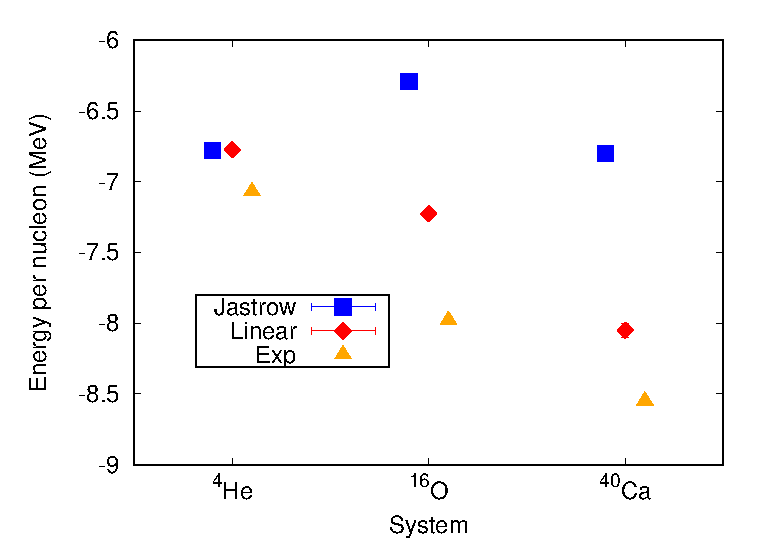
\includegraphics[width=0.7\textwidth]{figures/energy_jaslin.eps}
   \caption{Binding energy calculations done with Jastrow correlations (\cite{gandolfi2007}) compared to Jastrow plus linear spin-isospin dependent correlations (\cite{gandolfi2014}) all compared to experimental results. All calculations were done with AFDMC and the AV6$'$ potential.}
   \label{fig:energy_jaslin}
\end{figure}
In Figure~\ref{fig:energy_jaslin} it is clear to see that the additional spin-isospin correlations are important for both systems larger than $^4$He.

\subsection{Quadratic Correlations}
In this project I have included correlations up to quadratic order which includes up to 4 nucleons begin correlated at once. When expanded to quadratic order the symmetrized product wave function, Equation~\ref{equ:prodpsi}, becomes
\begin{equation}
   \begin{split}
      \ket{\psi_T}_\text{quad} = \Bigg[\prod\limits_{i<j}&f_c(r_{ij})\Bigg] \Bigg[1+\fOpij \\
         & + \frac{1}{2}\fOpij\fOqklquad \Bigg] \ket{\phi}.
   \end{split}
   \label{equ:fullquadcorr}
\end{equation}
The subscripts on the sums, which describe which correlations are allowed, can be hard to visualize and so these correlation diagrams are useful.
\begin{figure}[h]
\newcommand\shift{2.0}
\newcommand\vshift{-1.5} %vertical shift
\newcommand\tshift{0.05} %tiny shift
\newcommand\sep{0.75}
   \centering
   \begin{tikzpicture}[>=latex,scale=1.0]
      \draw (-2*\sep,\sep/2.0) node{\large Allowed};
      \draw (-2*\sep,\sep/2.0+\vshift) node{\large Not Allowed};

      \filldraw[black] (0*\shift,0)          circle (2pt) node[anchor=east] {\large j};
      \filldraw[black] (0*\shift,\sep)       circle (2pt) node[anchor=east] {\large i};
      \filldraw[black] (0*\shift+\sep,0)     circle (2pt) node[anchor=west] {\large l};
      \filldraw[black] (0*\shift+\sep,\sep)  circle (2pt) node[anchor=west] {\large k};
      \draw[black, ultra thick] (0*\shift,\sep) -- (0*\shift,0); %i-j
      \draw[black, ultra thick] (0*\shift+\sep,\sep) -- (0*\shift+\sep, 0); %k-l

      \filldraw[black] (1*\shift,0)          circle (2pt) node[anchor=east] {\large k};
      \filldraw[black] (1*\shift,\sep)       circle (2pt) node[anchor=east] {\large i};
      \filldraw[black] (1*\shift+\sep,0)     circle (2pt) node[anchor=west] {\large l};
      \filldraw[black] (1*\shift+\sep,\sep)  circle (2pt) node[anchor=west] {\large j};
      \draw[black, ultra thick] (1*\shift,\sep) -- (1*\shift+\sep,\sep); %i-j
      \draw[black, ultra thick] (1*\shift,0) -- (1*\shift+\sep,0); %k-l

      \filldraw[black] (2*\shift,0)          circle (2pt) node[anchor=east] {\large l};
      \filldraw[black] (2*\shift,\sep)       circle (2pt) node[anchor=east] {\large i};
      \filldraw[black] (2*\shift+\sep,0)     circle (2pt) node[anchor=west] {\large j};
      \filldraw[black] (2*\shift+\sep,\sep)  circle (2pt) node[anchor=west] {\large k};
      \draw[black, ultra thick] (2*\shift,\sep) -- (2*\shift+\sep,0); %i-j
      \draw[black, ultra thick] (2*\shift+\sep,\sep) -- (2*\shift,0); %k-l

      \filldraw[black] (3*\shift,0)          circle (2pt) node[anchor=east] {\large j};
      \filldraw[black] (3*\shift,\sep)       circle (2pt) node[anchor=east] {\large i,k};
      \filldraw[black] (3*\shift+\sep,0)     circle (2pt) node[anchor=west] {\large };
      \filldraw[black] (3*\shift+\sep,\sep)  circle (2pt) node[anchor=west] {\large l};
      \draw[black, ultra thick] (3*\shift,\sep) -- (3*\shift,0); %i-j
      \draw[black, ultra thick] (3*\shift,\sep) -- (3*\shift+\sep,\sep); %k-l

      \filldraw[black] (4*\shift,0)          circle (2pt) node[anchor=east] {\large k};
      \filldraw[black] (4*\shift,\sep)       circle (2pt) node[anchor=east] {\large i};
      \filldraw[black] (4*\shift+\sep,0)     circle (2pt) node[anchor=west] {\large j,l};
      \filldraw[black] (4*\shift+\sep,\sep)  circle (2pt) node[anchor=west] {\large };
      \draw[black, ultra thick] (4*\shift,\sep) -- (4*\shift+\sep,0); %i-j
      \draw[black, ultra thick] (4*\shift,0) -- (4*\shift+\sep,0); %k-l

      \filldraw[black] (2*\shift,\vshift)             circle (2pt) node[anchor=east] {\large j,l};
      \filldraw[black] (2*\shift,\sep+\vshift)        circle (2pt) node[anchor=east] {\large i,k};
      \filldraw[black] (2*\shift+\sep,\vshift)        circle (2pt) node[anchor=west] {\large };
      \filldraw[black] (2*\shift+\sep,\sep+\vshift)   circle (2pt) node[anchor=west] {\large };
      \draw[black, ultra thick] (2*\shift-\tshift,\sep+\vshift) -- (2*\shift-\tshift,\vshift); %i-j
      \draw[black, ultra thick] (2*\shift+\tshift,\sep+\vshift) -- (2*\shift+\tshift,\vshift); %k-l
   \end{tikzpicture}
   \caption{Diagrams used to visualize which correlations are included in the quadratic correlations in Equation~\ref{equ:fullquadcorr}.}
   \label{fig:quaddiagrams}
\end{figure}
All pair correlations are included in this wave function except pairs that are directly correlated with themselves, e.g. $\mathcal{O}_{23}\mathcal{O}_{23}$, where $\mathcal{O}_{ij}$ is a product of single particle operators such as $\si\cdot\sj$ and $\mathcal{O}_{ij}=\mathcal{O}_{ji}$ due to the operators on different particles operating in different Hilbert spaces. For correlations where the same particle is included twice, the correlation operators do not commute and that term must be explicitly symmetrized. Currently in Equation~\ref{equ:fullquadcorr} and in the code all quadratic terms are symmetrized, e.g. the correlation $\mathcal{O}_{12}\mathcal{O}_{34}$ is symmetrized as $\frac{1}{2}\left(\mathcal{O}_{12}\mathcal{O}_{34}+\mathcal{O}_{34}\mathcal{O}_{12}\right)$, even though only terms like $\mathcal{O}_{12}\mathcal{O}_{13}$ need this explicit symmetrization. This adds needless calculation time, but as I'll show, these terms don't seem to be significant and can be omitted completely.

If the exponentially correlated wave function, Equation~\ref{equ:exppsi}, is expanded in the typical way, i.e. $\exp(A) = 1 + A + \frac{1}{2}A^2 + \ldots$, then the quadratic correlations for the exponential wave function become
\begin{equation}
   \begin{split}
      \ket{\psi_T}_\text{exp\_quad} = \Bigg[\prod\limits_{i<j}&f_c(r_{ij})\Bigg] \Bigg[1+\fOpij \\
         & + \frac{1}{2}\fOpij\fOqklexpquad \Bigg] \ket{\phi}.
   \end{split}
   \label{equ:expquadcorr}
\end{equation}
Unlike the quadratic correlations derived from the symmetrized product this wave function includes all of the the terms in Figure~\ref{fig:quaddiagrams}. There is not a large difference between these wave functions up to quadratic order and for here forward all references to quadratic correlations will refer to the expansion from the symmetrized product wave function.

Another way to include quadratic correlations is to only include terms that do not correlate the same particle twice leaving only independent pair correlations. This is the same whether you start from the exponentially correlated or the symmetrized product wave function and it can be written as
\begin{equation}
   \begin{split}
      \ket{\psi_T}_\text{ip} = \Bigg[\prod\limits_{i<j}&f_c(r_{ij})\Bigg] \Bigg[1+\fOpij \\
      & + \fOpij\fOqklip \Bigg] \ket{\phi}
   \end{split}
   \label{equ:ipquadcorr}
\end{equation}
and the independent pair sum can be visualized as in Figure~\ref{fig:ipdiagrams}.
\begin{figure}[h]
\newcommand\shift{2.2}
\newcommand\vshift{-1.5} %vertical shift
\newcommand\tshift{0.05} %tiny shift
\newcommand\sep{0.75}
   \centering
   \begin{tikzpicture}[>=latex,scale=1.0]
      \draw (-3*\sep,\sep/2.0) node{\large Allowed};
      \draw (-3*\sep,\sep/2.0+\vshift) node{\large Not Allowed};

      \filldraw[black] (0*\shift,0)          circle (2pt) node[anchor=east] {\large j};
      \filldraw[black] (0*\shift,\sep)       circle (2pt) node[anchor=east] {\large i};
      \filldraw[black] (0*\shift+\sep,0)     circle (2pt) node[anchor=west] {\large l};
      \filldraw[black] (0*\shift+\sep,\sep)  circle (2pt) node[anchor=west] {\large k};
      \draw[black, ultra thick] (0*\shift,\sep) -- (0*\shift,0); %i-j
      \draw[black, ultra thick] (0*\shift+\sep,\sep) -- (0*\shift+\sep, 0); %k-l

      \filldraw[black] (1*\shift,0)          circle (2pt) node[anchor=east] {\large k};
      \filldraw[black] (1*\shift,\sep)       circle (2pt) node[anchor=east] {\large i};
      \filldraw[black] (1*\shift+\sep,0)     circle (2pt) node[anchor=west] {\large l};
      \filldraw[black] (1*\shift+\sep,\sep)  circle (2pt) node[anchor=west] {\large j};
      \draw[black, ultra thick] (1*\shift,\sep) -- (1*\shift+\sep,\sep); %i-j
      \draw[black, ultra thick] (1*\shift,0) -- (1*\shift+\sep,0); %k-l

      \filldraw[black] (2*\shift,0)          circle (2pt) node[anchor=east] {\large l};
      \filldraw[black] (2*\shift,\sep)       circle (2pt) node[anchor=east] {\large i};
      \filldraw[black] (2*\shift+\sep,0)     circle (2pt) node[anchor=west] {\large j};
      \filldraw[black] (2*\shift+\sep,\sep)  circle (2pt) node[anchor=west] {\large k};
      \draw[black, ultra thick] (2*\shift,\sep) -- (2*\shift+\sep,0); %i-j
      \draw[black, ultra thick] (2*\shift+\sep,\sep) -- (2*\shift,0); %k-l

      \filldraw[black] (0*\shift,\vshift)          circle (2pt) node[anchor=east] {\large j};
      \filldraw[black] (0*\shift,\sep+\vshift)       circle (2pt) node[anchor=east] {\large i,k};
      \filldraw[black] (0*\shift+\sep,\vshift)     circle (2pt) node[anchor=west] {\large };
      \filldraw[black] (0*\shift+\sep,\sep+\vshift)  circle (2pt) node[anchor=west] {\large l};
      \draw[black, ultra thick] (0*\shift,\sep+\vshift) -- (0*\shift,\vshift); %i-j
      \draw[black, ultra thick] (0*\shift,\sep+\vshift) -- (0*\shift+\sep,\sep+\vshift); %k-l

      \filldraw[black] (1*\shift,\vshift)          circle (2pt) node[anchor=east] {\large k};
      \filldraw[black] (1*\shift,\sep+\vshift)       circle (2pt) node[anchor=east] {\large i};
      \filldraw[black] (1*\shift+\sep,\vshift)     circle (2pt) node[anchor=west] {\large j,l};
      \filldraw[black] (1*\shift+\sep,+\vshift)  circle (2pt) node[anchor=west] {\large };
      \draw[black, ultra thick] (1*\shift,\sep+\vshift) -- (1*\shift+\sep,\vshift); %i-j
      \draw[black, ultra thick] (1*\shift,\vshift) -- (1*\shift+\sep,\vshift); %k-l

      \filldraw[black] (2*\shift,\vshift)             circle (2pt) node[anchor=east] {\large j,l};
      \filldraw[black] (2*\shift,\sep+\vshift)        circle (2pt) node[anchor=east] {\large i,k};
      \filldraw[black] (2*\shift+\sep,\vshift)        circle (2pt) node[anchor=west] {\large };
      \filldraw[black] (2*\shift+\sep,\sep+\vshift)   circle (2pt) node[anchor=west] {\large };
      \draw[black, ultra thick] (2*\shift-\tshift,\sep+\vshift) -- (2*\shift-\tshift,\vshift); %i-j
      \draw[black, ultra thick] (2*\shift+\tshift,\sep+\vshift) -- (2*\shift+\tshift,\vshift); %k-l
   \end{tikzpicture}
   \caption{Diagrams used to visualize which correlations are included in the independent pair quadratic correlations in Equation~\ref{equ:ipquadcorr}.}
   \label{fig:ipdiagrams}
\end{figure}
All terms where a particle is included twice in the correlation are ignored, as a results, all correlation operators commute and the correlations are explicitly symmetric. Neither of these correlations maintains cluster decomposability, however an effort to build an antisymmetric and cluster decomposable wave function from the exponentially correlated wave function will be discussed later.

The energy and it's uncertainty are used to judge the convergence of a propagated wave function in QMC and so a good wave function needs to be able to reproduce known binding energies. To this end I have calculated binding energies with the linear, quadratic, and independent pair (IP) quadratic correlations derived from the symmetrized product for $^4$He, $^{16}$O, $^{40}$Ca, and symmetric nuclear matter (SNM) at saturation density, $\rho_0=0.16$ fm$^{-3}$, in a period box with 28 particles. The energy per particle for nuclei is plotted in Figure~\ref{fig:energies} and the specific energies can be found in Table~\ref{tab:energies}.
\begin{figure}[h!]
   \centering
   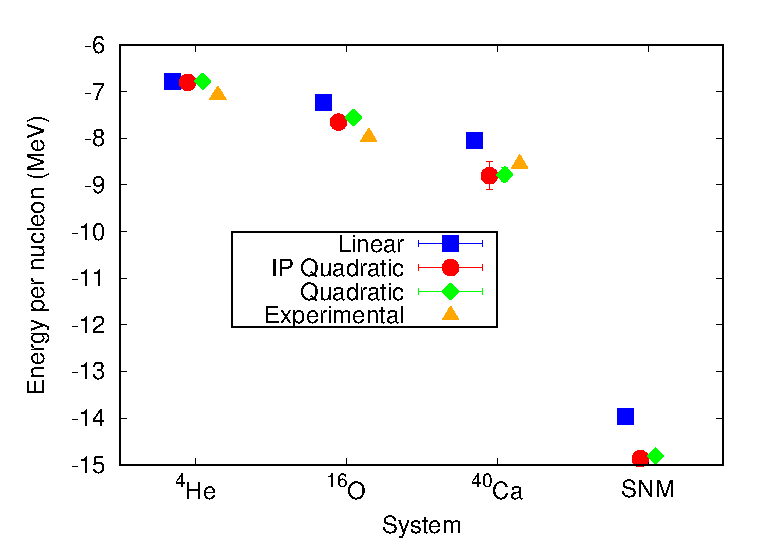
\includegraphics[width=0.7\textwidth]{figures/energy.eps}
   \caption{Energy per particle for small and medium closed shell nuclei with no Coulomb interaction calculated with the AFDMC method with the AV6$'$ interaction. Each calculations was done with the linear, IP quadratic, and quadratic correlations. Energies are compared to experimental values where available and the statistical uncertainties are included. The variational parameters were reoptimized for each wave function the $^4$He calculations, however the $^{16}$O, $^{40}$Ca, and SNM calculations were done starting with VMC trial wave functions with linear correlations.}
   \label{fig:energies}
\end{figure}
\begin{table}[htb]
   \centering
   \begin{tabular}{ccccc}
      \hline\hline
      System & Linear & Ind-Pair & Quadratic & Experimental \\
      \hline
      $^4${He}    & -6.785(10)   & -6.798(8) & -6.778(8)    & -7.074 \\   
      $^{16}${O}  & -7.23(6)     & -7.65(9)  & -7.55(8)     & -7.98  \\   
      $^{40}${Ca} & -8.05(8)     & -8.8(3)   & -8.78(15)    & -8.55  \\
      SNM         & -13.97(3)    & -14.87(4) & -14.70(11)   &        \\
      \hline\hline
   \end{tabular}
   \caption{Energy per particle from AFDMC calculations with no Coulomb interaction with the AV6$'$ interaction. Each calculations was done with the linear, independent pair, and quadratic correlations. Energies are compared to experimental values where available and the statistical uncertainties are included.}
   \label{tab:energies}
\end{table}
All calculations were done with trial wave functions coming from VMC calculations with linear correlations, except for $^4$He, which was performed by reoptimizing the variational parameters for each set of correlations. This was done due to the complexity of optimizing the parameters for large systems. Like with the addition of Jastrow correlations in Figure~\ref{fig:energy_jaslin}, all systems larger than $^4$He decreased in energy with additional correlations, while the binding energy for $^4$He was the same to within uncertainties. In addition, the energies for all systems are identical to within uncertainties for the quadratic and IP quadratic correlations, indicating that the IP correlations capture most of the relevant physics. As a result any further references to quadratic correlations will be referring to the IP quadratic correlations, as these correlations are computationally less expensive, unless a distinction is made otherwise. The percent decrease in energy for $^{16}$O and $^{40}$Ca when adding linear correlations is 15\% and 18\% respectively. When adding quadratic correlations the energies decrease an additional 6\% and 9\% respectively. This indicates that each successive term in the expansion decreases in importance. It is important to note that these calculations were done with the AV6$'$ potential, which is a limited 2-nucleon potential. We do not expect our energies to be equal to experiment due to the lack of the full 2-body, and a complete lack of the 3-body force. The AV6$'$ potential has been used to simplify the calculations and to look for qualitative improvements caused by the additional correlations. Some calculations have been done using more sophisticated potentials with the quadratic correlations, and those results will be shown later.

The energies above are calculated with the AFDMC method. The fixed phase approximation is used to solve the Fermi sign problem within AFDMC, and as such the energies are not constrained by the variational principle, i.e. the energies are not strict upper bounds to the ground state energy, as evidenced by the results for $^{40}$Ca, which is actually overbound. The lack of an upper bound prevents us to say strictly that the decrease in energy is because of an improvement in the trial wave function. However, all calculations were first done with the VMC method, which does provide an upper bound constraint. As can be seen in Figure~\ref{fig:energies_vmc} and Table~\ref{tab:energies_vmc}, the same conclusions found with the AFDMC calculations are also found with the VMC calculations, as we can say that the quadratic wave functions are actually an improvement.

\begin{figure}[h!]
   \centering
   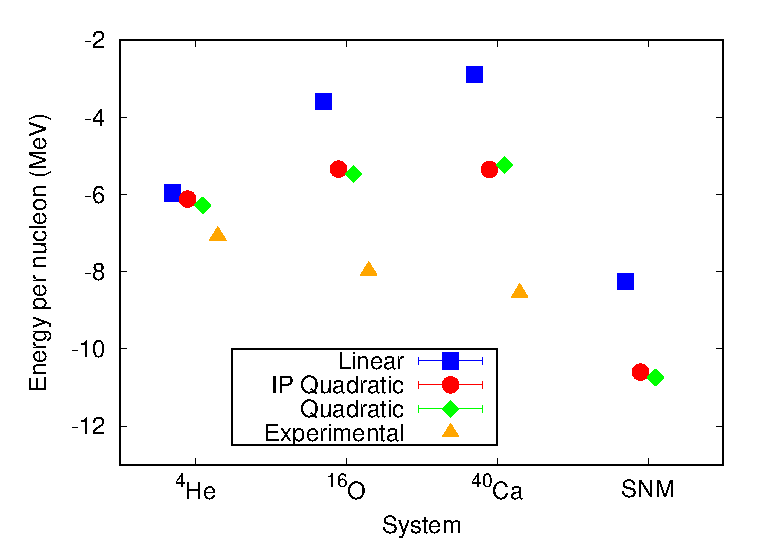
\includegraphics[width=0.7\textwidth]{figures/energy_vmc.eps}
   \caption{Energy per particle for small and medium closed shell nuclei with no Coulomb interaction calculated with the VMC method with the AV6$'$ interaction. Each calculations was done with the linear, independent pair, and quadratic correlations. Energies are compared to experimental values where available and the statistical uncertainties are included. Unlike the above results, calculated with the AFDMC method, these VMC results are an upper bound to the ground state energy.}
   \label{fig:energies_vmc}
\end{figure}
\begin{table}[htb]
   \centering
   \begin{tabular}{ccccc}
      \hline\hline
      System & Linear & Ind-Pair & Quadratic & Experimental \\
      \hline
      $^4${He}    & -5.955(10)   & -6.113(8) & -6.275(5)    & -7.074 \\   
      $^{16}${O}  & -3.581(3)    & -5.338(3) & -5.463(3)    & -7.98  \\   
      $^{40}${Ca} & -2.88(5)     & -5.35(5)  & -5.23(5)     & -8.55  \\
      SNM         & -8.25(4)     & -10.60(3) & -10.74(2)    &        \\
      \hline\hline
   \end{tabular}
   \caption{Energy per particle from VMC calculations with no Coulomb interaction with the AV6$'$ interaction. Unlike the AFDMC results, these VMC results provide an upper bound to the energy. Each calculations was done with the linear, independent pair, and quadratic correlations. Energies are compared to experimental values where available and the statistical uncertainties are included.}
   \label{tab:energies_vmc}
\end{table}

There is a significant decrease in energy with the addition of the quadratic correlations, however, there is an additional cost to calculating these additional terms. I have calculated a scaling factor, which is the ratio of times taken to calculate a given block of code, including the propagation of walkers spatial and spin components as well as the calculation of the energies, for linear compared to linear plus quadratic correlations. A scaling factor of 2 would mean that the calculation took twice as long with the quadratic correlations as it did without. The scaling factors are plotted in Figure~\ref{fig:scaling} and the specific values are in Table~\ref{tab:scaling}.
\begin{figure}[h!]
   \centering
   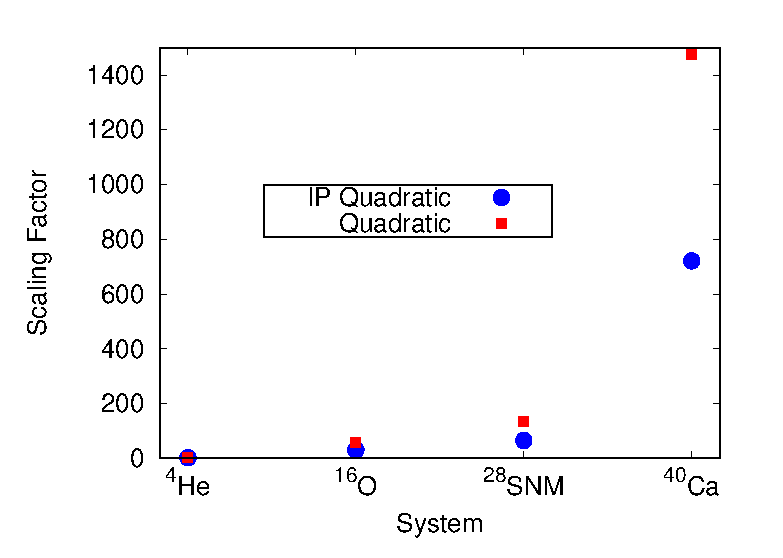
\includegraphics[width=0.7\textwidth]{figures/scaling.eps}
   \caption{Scaling factors calculated as the ratio of times taken to calculate a given block of code for linear and linear plus quadratic correlations.}
   \label{fig:scaling}
\end{figure}
\begin{table}[htb]
   \centering
   \begin{tabular}{ccccc}
      \hline \hline
       & $^{4}$He & $^{16}$O & SNM(28) & $^{40}$Ca \\
      \hline
      IP Quadratic & 1.73 & 30.7 & 64.8 & 720.9 \\
      Quadratic & 2.00 & 58.8 & 133.6 & 1473.9 \\
      \hline \hline
   \end{tabular}
   \caption{Same scaling factors that are calculated in Figure~\ref{fig:scaling}.}
   \label{tab:scaling}
\end{table}
The scaling for the quadratic correlations is about twice that of the IP quadratic correlations. This is due to the explicit symmetrization that is done for each quadratic term in the quadratic correlations. This could be decreased if commuting terms were not symmetrized, however as noted before the IP quadratic correlations seem to capture the important physics, and so all future calculations with quadratic correlations will be using the IP correlations. The IP correlations all commute and so no explicit symmetrization is needed. A typical AFDMC calculation using only linear correlations for $^{16}$O with 1000 walkers takes on the order of a tens of CPU hours and a similar calculation for $^{40}$Ca takes on the order of hundreds of CPU hours.

The number of quadratic terms in the IP correlations given $A$ particles is
\begin{equation}
   N_\text{ip}=\frac{A(A-1)(A-2)(A-3)}{8}.
\end{equation}
For the fully quadratic wave function the number of terms given $A$ particles is
\begin{equation}
   N_\text{quad}=\frac{A(A-1)}{2}\left(\frac{A(A-1)}{2}-1\right),
\end{equation}
where $A(A-1)/2$ is the number of possible pairs made from $A$ particles. If the fully quadratic correlations are not explicitly symmetrized for the IP terms then this reduces to $N_\text{quad}-N_\text{ip}$. In Figure~\ref{fig:scaling_theory} I have plotted the number of terms for the independent pair, fully quadratic, and fully quadratic correlations without symmetrizing the IP terms.
\begin{figure}[h!]
   \centering
   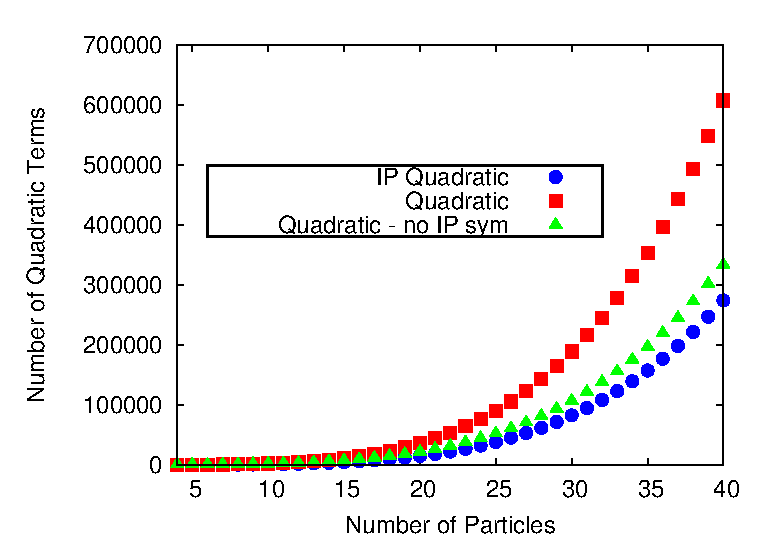
\includegraphics[width=0.7\textwidth]{figures/scaling_theory.eps}
   \caption{Number of terms in the quadratic correlations for the IP, quadratic, and quadratic correlations without explicit symmetrization of the IP terms.}
   \label{fig:scaling_theory}
\end{figure}

In recent years efforts have been made to fit infinite matter saturation properties with microscopic nuclear interactions (\cite{drischler2017}). Calculations of energies near saturation using AFDMC have not been able to fit known saturation properties. I have done calculations of symmetric nuclear matter near saturation with and without quadratic correlations, using only the AV6$'$ 2-body interaction and have compared these results to known saturation properties in Figure~\ref{fig:saturation}. Though 3N forces will surely be needed to obtain a good fit, it is clear that improved correlations are also going to be needed.
\begin{figure}[h!]
   \centering
   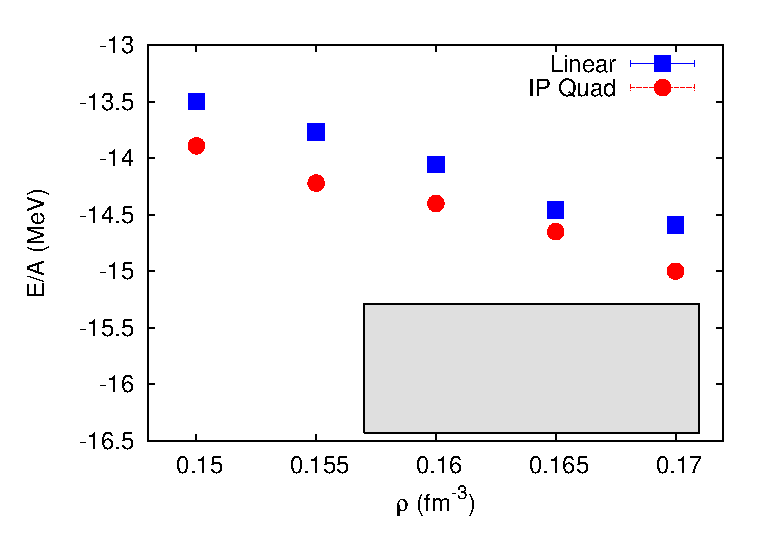
\includegraphics[width=0.7\textwidth]{figures/saturation.eps}
   \caption{Energy calculations done using the AV6$'$ potential with linear and quadratic correlations. The gray box is the same empirical saturation region used in \cite{drischler2017}, $\rho_0 = 0.164 \pm 0.007$ fm$^{-3}$ and $E/A=-15.86 \pm 0.57$ MeV.}
   \label{fig:saturation}
\end{figure}

\subsection{Calculating the Two-Body Operators}
When calculating expectation values with the additional two-body operators of the quadratic correlations, the scaling will increase from $O(A^4)$ to $O(A^6)$ for the calculation of the energy and from $O(A^2)$ to $O(A^4)$ for the calculation of the trial wave function alone. This can be quite expensive, especially for large systems. As a result we have used a technique to reduce the number of calculations by performing recurring pieces of the calculations only once at the beginning. Though this doesn't decrease the polynomial scaling it does decrease the factor in front of the polynomial scaling.

The Slater Determinant is the base ingredient to calculating the trial wave function. The Slater matrix is defined as
\begin{equation}
   S = \begin{pmatrix}
      \braket{\alpha_1}{\r_1,s_1} & \braket{\alpha_1}{\r_2,s_2} & \ldots & \braket{\alpha_1}{\r_A,s_A} \\
      \braket{\alpha_2}{\r_1,s_1} & \braket{\alpha_2}{\r_2,s_2} & \ldots & \braket{\alpha_2}{\r_A,s_A} \\
      \vdots & \vdots & \ddots & \vdots \\
      \braket{\alpha_A}{\r_1,s_1} & \braket{\alpha_A}{\r_2,s_2} & \ldots & \braket{\alpha_A}{\r_A,s_A}
   \end{pmatrix},
\end{equation}
where each matrix element will be written as
\begin{equation}
   S_{\alpha i} = \braket{\alpha}{\r_i,s_i}.
\end{equation}
This can be written in terms of the spin-isospin basis as
\begin{equation}
   S_{\alpha i} = \sum\limits_{\gamma=1}^4 \braket{\alpha}{\r_i \chi_\gamma}\braket{\chi_\gamma}{s_i}.
\end{equation}
where $\r_i$ and $s_i$ are the positions and spin-isospin configurations of the system, and $\ket{\alpha}$ contains the radial part of the wave function and the spherical harmonics that give the proper angular momentum to each state. The $\ket{\chi_\gamma}$ basis is given in terms of $\ket{p\uparrow}$, $\ket{p\downarrow}$, $\ket{n\uparrow}$, and $\ket{n\downarrow}$ as
\begin{equation}
\begin{split}
   \ket{\chi_1} &= \ket{\left(1,0,0,0\right)} \\
   \ket{\chi_2} &= \ket{\left(0,1,0,0\right)} \\
   \ket{\chi_3} &= \ket{\left(0,0,1,0\right)} \\
   \ket{\chi_4} &= \ket{\left(0,0,0,1\right)}.
\end{split}
\end{equation}

The Slater matrix is updated once for every single-body operator and twice for every two-body operator using the identity
\begin{equation}
   \det{\left(S^{-1}S'\right)} = \frac{\det{S'}}{\det S},
   \label{equ:matrixid}
\end{equation}
where $S'$ is the Slater matrix that has been updated due to the operation of a single-body operator.

Using the identity in Equation~\ref{equ:matrixid} allows us to calculate the product $S^{-1}S''$, where $S''$ represents the Slater matrix with only the $i$ and $j$ columns updated. The product $S^{-1}S$ would give the identity matrix and so $S^{-1}S''$ is the identity matrix everywhere except for the columns $i$ and $j$
\begin{equation}
   S^{-1}S'' = 
   \begin{pmatrix}
      1 & 0 & \ldots & \bra{\alpha_1}\mathcal{O}_i\ket{\r_i,s_i} & \ldots & \bra{\alpha_1}\mathcal{O}_j\ket{\r_j,s_j} & \ldots & 0 & 0 \\
      0 & 1 & \ldots & \bra{\alpha_2}\mathcal{O}_i\ket{\r_i,s_i} & \ldots & \bra{\alpha_2}\mathcal{O}_j\ket{\r_j,s_j} & \ldots & 0 & 0 \\
      \vdots & \vdots & \ddots & \vdots & \ddots & \vdots & \ddots & \vdots & \vdots \\
      0 & 0 & \ldots & \bra{\alpha_A}\mathcal{O}_i\ket{\r_i,s_i} & \ldots & \bra{\alpha_A}\mathcal{O}_j\ket{\r_j,s_j} & \ldots & 0 & 1 \\
   \end{pmatrix}.
\end{equation}
The determinant is then equal to the determinant of the submatrix given by keeping only the elements $\left(S^{-1}S''\right)_{mn}$ where $m$ and $n$ are both of the changed columns
\begin{equation}
   \det{S^{-1}S''} =
   \det\begin{pmatrix}
      \bra{\alpha_i}\mathcal{O}_i\ket{\r_i,s_i} & \bra{\alpha_i}\mathcal{O}_j\ket{\r_j,s_j} \\
      \bra{\alpha_j}\mathcal{O}_i\ket{\r_i,s_i} & \bra{\alpha_j}\mathcal{O}_j\ket{\r_j,s_j} \\
   \end{pmatrix}.
\end{equation}

In practice the calculation of a two-body operator $\mathcal{O}_{ij}=\mathcal{O}_i\mathcal{O}_j$ is calculated as
\begin{equation}
   \frac{\bra{\Phi}\mathcal{O}_{ij}\ket{RS}}{\braket{\Phi}{RS}} = \sum\limits_{\gamma=1}^4\sum\limits_{\delta=1}^4 d_{2b}(\chi_\gamma,\chi_\delta,ij)\bra{\chi_\gamma\chi_\delta}\mathcal{O}_{ij}\ket{s_is_j},
   \label{equ:d2bdef}
\end{equation}
where $R=\{\r_1,\ldots,\r_A\}$ and $S=\{s_1,\ldots,s_A\}$ are the spatial and spin-isospin configurations and
\begin{equation}
   d_{2b}(\chi_\gamma,\chi_\delta,ij)=\frac{\langle\Phi|R,s_1,\ldots,s_{i-1},\chi_\gamma,s_{i+1},\ldots,s_{j-1},\chi_\delta,s_{j+1},\ldots,s_A\rangle}{\langle \Phi|RS\rangle}.
\end{equation}
Note that as part of the update the basis states $\chi_\gamma$ and $\chi_\delta$ have replaced the spin-isospin configurations $s_i$ and $s_j$ respectively.

To reduce the number of calculations done in the inner loops of the calculation the matrix $P_{\chi,ij}$ is defined and precalculated as
\begin{align}
   P_{\chi_\gamma,ij} &=\sum_\alpha S^{-1}_{j\alpha}S_{\alpha i}(s_i\leftarrow \chi_\gamma), \\
   P_{\chi_\delta,ij} &=\sum_\alpha S^{\prime\;-1}_{j\alpha}S^\prime_{\alpha i}(s_j\leftarrow \chi_\delta).
\end{align}
The $d_{2b}$ distribution can then be written as
\begin{equation}
   d_{2b}(\chi_\gamma,\chi_\delta,ij)=\det\begin{pmatrix}P_{\chi_\gamma,ii} & P_{\chi_\gamma,ij} \\ P_{\chi_\delta,ji} & P_{\chi_\delta,jj}\end{pmatrix},
\end{equation}
and thus the $d_{2b}$ can be precalculated and multiplied by each operator expectation value $\bra{\chi_\gamma\chi_\delta}\mathcal{O}_{ij}\ket{s_is_j}$ from Equation~\ref{equ:d2bdef}.

This description has been for 2-body operators, however the quadratic operators involve 4-body operators for the correlations of the trial wave function, and 6-body operators for the calculations of the energy. This method can also be extended to $n$-body operators by updating the $P$ matrix to use the previously updated Slater matrices
\begin{equation}
   P_{\chi_\eta,mn}=\sum_\alpha S^{\prime\prime\;-1}_{n\alpha}S^{\prime\prime}_{\alpha m}(s_m\leftarrow \chi_\eta),
\end{equation}
where each iteratively updated matrix $S'$ is calculated from the last $S$ as
\begin{align}
   S^{\prime}_{\alpha m}(s_m) = \left\{
   \begin{array}{cc}
      S_{\alpha m} & m \ne i\\
      \langle\alpha|\mathcal O_i|\mathbf{r}_i\,s_i\rangle  & m = i
   \end{array} .
   \right.
\end{align}
The updated inverse matrix is calculated by again using the identity in Equation~\ref{equ:matrixid}, expanding both sides and grouping like terms, noting that $S''_{mi} = S'_{mi}$ when $j\ne i$. The next iteration of the updated inverse matrix $S'^{-1}$ is calculated as
\begin{equation}
S'^{-1}_{jn} = \left \{
\begin{array}{cc}
S^{-1}_{jn} -\frac{\sum_m S^{-1}_{jm}S'_{mi}}{\sum_\ell S^{-1}_{i\ell}
S'_{\ell i}} S^{-1}_{in}  & j \ne i\\
\frac{S^{-1}_{in}}{\sum_m S^{-1}_{im}S'_{mi}} & j = i\\
\end{array}
\right . \,.
\end{equation}

To calculate the wave function in Equation~\ref{equ:linearcorr} with only linear correlations the correlation operators are first acted on the spin-isospin basis states which are then summed together with the $d_{2b}$ as
\begin{equation}
   \sum\limits_{\chi_\gamma,\chi_\delta}d_{2b}(\chi_\gamma,\chi_\delta,ij)\langle\chi_\gamma,\chi_\delta|f_{ij}^p\mathcal{O}_{ij}^p|s_i s_j\rangle.
\end{equation}
The potential introduces two additional operators and so the expectation value of the potential with the linear wave function is calculated as $(\mathbb{1}+\mathcal{O}^c_{ij})\mathcal{O}^p_{kl}$ where $\mathcal{O}^c$ and $\mathcal{O}^p$ are the correlation and potential operators respectively and can be four distinct operators. This calculation is done by first updating the $P$ matrix twice, once for each of $\mathcal{O}^c_i$ and $\mathcal{O}^c_j$ where $\mathcal{O}_{ij}=\mathcal{O}_i\mathcal{O}_j$. The determinant in Equation~\ref{equ:d2bdef} is then calculated using the updated $d''_{2b}$.

Both versions of the quadratic correlations in Equations~\ref{equ:fullquadcorr} and \ref{equ:ipquadcorr} have the form $\mathbb{1} + \mathcal{O}^c_{ij} + \mathcal{O}^c_{ij}\mathcal{O}_{kl}$. The first is exactly the linear correlations and are calculated in the same way as described above. The quadratic operators looks like the potential operator with linear correlations with $\mathcal{O}^c_{ij}\mathcal{O}^p_{kl} \rightarrow \mathcal{O}^c_{ij}\mathcal{O}^c_{kl}$ and so the same method can be followed as described before by updating the $P$ matrix twice. The number of operations required for the linear correlations scales as $O(A^2)$ while the quadratic correlations, as well as the expectation value of the potential with linear correlations, scales as $O(A^4)$.

The expectation value of the potential as calculated with the quadratic correlations takes the form $\left(\mathbb{1} + \mathcal{O}^c_{ij} + \mathcal{O}^c_{ij}\mathcal{O}_{kl}\right)\mathcal{O}^p_{mn}$. The only piece that is not similar to previous descriptions is the $\mathcal{O}^c_{ij}\mathcal{O}^c_{kl}\mathcal{O}^p_{mn}$ piece. This can be calculated by using four distinct updates of the $P$ matrix, one for each of the four correlations operators. The updates are first done for the $\mathcal{O}^c_{ij}$ operators after which two additional updates are performed for the $\mathcal{O}^c_{kl}$ operators. This is used to calculate the expectation value of the $\mathcal{O}^p_{mn}$ operators. The scaling to calculate the expectation value of the potential with quadratic correlations is $O(A^6)$.

Additional details about the quadratic correlations and how the operator updates are performed can be found in our recent paper \cite{lonardoni2018}.

\subsection{Quadratic Correlations with NN and 3N $\chi$EFT Potentials}
The results presented above have been done with the simplified AV6$'$ NN potential. This choice was made to reduce the computational cost of testing the improved correlations. The new quadratic correlations have also been used with more sophisticated potentials, namely, those developed in the $\chi$EFT framework. We have done preliminary calculations with the $\chi$EFT potential up to N$^2$LO in the chiral expansion. Higher orders of the chiral expansion are still inaccessible to QMC calculations due to their non-locality. We have obtained preliminary results (Diego Lonardoni, private communication, 2019) of binding energy calculations for $^4$He, $^{16}$O, and SNM with 28 particles in a periodic box at saturation density. Both the VMC and AFDMC preliminary results are shown in Table~\ref{tab:chiquad}.
\begin{table}[htb]
   \centering
   \begin{tabular}{llccc}
      \hline
      Calculation & Correlations & $^4$He & $^{16}$O & SNM \\
      \hline
      VMC   & Linear       & $-5.86(1)$ & $-1.08(1)$ & $1.56(5)$ \\
      VMC   & IP Quadratic & $-$        & $-4.03(4)$ & $-$ \\
      VMC   & Quadratic    & $-6.72(1)$ & $-3.95(4)$ & $-$ \\
      \hline
      AFDMC & Linear       & $-6.89(2)$ & $-5.74(4)$ & $-9.5(1)$ \\
      AFDMC & IP Quadratic & $-$        & $-7.3(2)$  & $-12.5(1)$ \\
      AFDMC & Quadratic    & $-6.91(2)$ & $-6.9(2)$  & $-12.6(1)$ \\
      \hline
   \end{tabular}
   \caption{Ground state energies of $^4$He, $^{16}$O, and SNM with 28 particles at saturation density, calculated with the VMC and AFDMC methods. All energies are reported as energy/nucleon in MeV. The trial wave functions are calculated with both 2- and 3-body correlations, where all three 2-body correlations were used. For all calculations the N$^2$LO local chiral potential with the $R_0 = 1$ fm cutoff as described in our paper (\cite{lonardoni2018}). Additional details about each calculation are given in the text. Not all possible calculations were performed, and dashes are places where data does not exist.}
   \label{tab:chiquad}
\end{table}
All calculations were done with 2- and 3-body correlations, however the 2-body correlations were varied to include the linear, IP quadratic, and the fully quadratic correlations. The potential used in these calculations was the local chiral potential expanded to N$^2$LO with a cutoff of $R_0=1$ fm. The $^4$He and SNM calculations were done with the $E\mathbb{1}$ parameterization, while the $^{16}$O calculations were done with the $E\tau$ parameterization as described in our paper \cite{lonardoni2018}. The $^4$He and $^{16}$O calculations included the coulomb force and were reoptimized for each set of correlations. Due to the computational cost of reoptimizing the variational parameters with the quadratic wave functions the AFDMC calculations for SNM were done using the trial wave function obtained from a VMC calculations with linear correlations. In addition the AFDMC calculations for SNM were done using the growth energy, which is a diagnostic tool which is similar to the local energy for small time steps. If the trial wave function was exactly the ground state and the offset energy $E_0$ the exact ground state energy, then the weights of the walkers would all be 1, regardless of the configuration. This leads to the definition of the growth energy
\begin{equation}
\left<E_G\right> = E_0-\frac{1}{\Delta\tau}\log{(\left<w\right>)}.
\end{equation}
More details on the growth energy are given in \cite{lynn2013}. All AFDMC calculation were performed with the constrained-path approximation. The 2-body operator structure of the N$^2$LO chiral interaction is the same as the AV7$'$ potential which adds the spin-orbit $\mathbf{L}\cdot\mathbf{S}$ term to the AV6$'$ interaction. It was shown in \cite{gandolfi2014} that the AV7$'$ potential provides less binding than the AV6$'$ potential for the systems shown here. This explains why the energies are slightly higher here than with the AV6$'$ results shown in the preceding sections. However, the decrease in energy between the linear and quadratic correlations is much larger when the 3-body interactions are included. The decrease in the $^{16}$O energy between linear correlations and IP quadratic correlations with only the AV6$'$ NN potential was 6\%, while the same system had a decrease of 27\% with the NN+3N N$^2$LO potential. This was expected as we expected the additional correlations to have a larger overlap with the 3-body force than the original linear correlations.

\subsection{Exponential Correlations}
From the wave function using the expansion up to quadratic terms it is clear that an improved trial wave function is necessary to describe the state of larger nuclei and nuclear matter. It was also shown in the previous sections that expanding the current wave functions described in Equations~\ref{equ:exppsi} and \ref{equ:prodpsi}, is not an efficient method to improve the wave function, as the cost of each additional term grows exponentially. However, another option is to evaluate the full wave function using a Monte Carlo sampling. The exponential wave function is written as
\begin{equation}
   \ket{\Psi_T} = \left[\prod\limits_{i<j}f_c(r_{ij})\right] e^{\sum\limits_{i<j,p}f_p(r_{ij})\Oijp} \ket{\Phi},
\end{equation}
which has the same operator form as the spin-isospin propagator used in AFDMC, where again, the operators are the AV6$'$ operators, $\si\cdot\sj$, $\ti\cdot\tj$, $\si\cdot\sj \ti\cdot\tj$, $S_{ij}$ and $S_{ij} \ti\cdot\tj$, where $S_{ij} = 3\si\cdot\hat{r}_{ij}\sj\cdot\hat{r}_{ij}-\si\cdot\sj$. These operators are written in terms of squared single particle operators, allowing for the Hubbard Stratanovich transformation to express the correlations in terms of a single particle operator and integrals over auxiliary fields, which are evaluated via Monte Carlo.

The correlation functions $f_p(r_{ij})$ are written in terms of symmetric matrices
\begin{equation}
\begin{split}
   \exp\left(\sum\limits_{i<j,p}f_p(r_{ij})\Oijp\right) = \exp&\left(\frac{1}{2}\sum\limits_{i\alpha,j\beta} \sigma_{i\alpha}A^{\sigma}_{i\alpha,j\beta}\sigma_{j\beta}\right. \\
      &\left. + \frac{1}{2}\sum\limits_{i\alpha,j\beta} \sigma_{i\alpha}A^{\sigma\tau}_{i\alpha,j\beta}\sigma_{j\beta}\ti\cdot\tj
      + \frac{1}{2}\sum\limits_{i,j} A^{\tau}_{i,j}\ti\cdot\tj\right),
\end{split}
\end{equation}
which can be written in terms of their eigenvalues and eigenvectors
\begin{align}
   &\sum\limits_{j\beta} A^{\sigma}_{i\alpha,j\beta}\psi^{\sigma}_{n,j\beta} = \lambda^{\sigma}_n\psi^{\sigma}_{n,i\alpha} \\
   &\sum\limits_{j\beta} A^{\sigma\tau}_{i\alpha,j\beta}\psi^{\sigma\tau}_{n,j\beta} = \lambda^{\sigma\tau}_n\psi^{\sigma\tau}_{n,i\alpha} \\
   &\sum\limits_{j} A^{\tau}_{i,j}\psi^{\tau}_{n,j} = \lambda^{\tau}_n\psi^{\tau}_{n,i}.
\end{align}
The correlations are then written in terms of squared single particle operators,
\begin{equation}
\begin{split}
   \exp\left(\sum\limits_{i<j,p}f_p(r_{ij})\Oijp\right) = \exp&\left(\frac{1}{2}\sum\limits_{n=1}^{3A} \left(O_{n}^{\sigma}\right)^2 \lambda_n^{\sigma}\right. \\
      & \left. + \frac{1}{2}\sum\limits_{\alpha=1}^{3}\sum\limits_{n=1}^{3A} \left(O_{n\alpha}^{\sigma\tau}\right)^2 \lambda_n^{\sigma\tau}
      + \frac{1}{2}\sum\limits_{\alpha=1}^{3}\sum\limits_{n=1}^{A} \left(O_{n\alpha}^{\tau}\right)^2 \lambda_n^{\tau}\right),
\end{split}
\end{equation}
where the operators are given by
\begin{equation}
\begin{split}
   O_{n}^{\sigma} &= \sum\limits_{j,\beta} \sigma_{j,\beta}\psi_{n,j,\beta}^{\sigma} \\
   O_{n\alpha}^{\sigma\tau} &= \sum\limits_{j,\beta} \tau_{j,\alpha}\sigma_{j,\beta}\psi_{n,j,\beta}^{\sigma\tau} \\
   O_{n\alpha}^{\tau} &= \sum\limits_{j} \tau_{j,\alpha}\psi_{n,j}^{\tau}.
\end{split}
\end{equation}
This can be written in a more compact form,
\begin{equation}
    \exp\left(\sum\limits_{i<j,p}f_p(r_{ij})\Oijp\right) = \exp\left(\frac{1}{2}\sum\limits_{n=1}^{15A} \left(O_{n}\right)^2 \lambda_n^{\sigma}\right).
\end{equation}
The Hubbard Stratanovich transformation is then used to write these as single particle operators and integrals over auxiliary fields, $x_n$. Ignoring commutator terms this can be written as
\begin{equation}
   \exp\left(\frac{1}{2}\sum\limits_{n=1}^{15A} \left(O_{n}\right)^2 \lambda_n^{\sigma}\right) = \prod\limits_{n=1}^{15A} \frac{1}{\sqrt{2\pi}}\int dx_n e^{-x_n^2/2}e^{\sqrt{\lambda_n}x_nO_n}.
\end{equation}

The auxiliary fields are then drawn from the Gaussian distribution, $\exp\left(-x_n^2/2\right)$ and the correlations can be written as
\begin{equation}
   \Psi_T(R,S) = \bra{RS}\prod\limits_{n=1}^{15A} \frac{1}{N} \sum\limits_{\{x_n\}}^N\frac{1}{\sqrt{2\pi}}e^{\sqrt{\lambda_n}x_nO_n}\ket{\Phi}.
\end{equation}
The $\{x_n\}$ are the set of 15$A$ auxiliary fields, one for each of the different 15$A$ operators.

Minimal success has been achieved with these correlations for light nuclei (\cite{bouadani2009_dissertation}), however there are large uncertainties that make this wave function currently infeasible to use. Removing these uncertainties could make this wave function a very useful tool for nuclear QMC as it can be systematically improved by increasing the number of samples of the auxiliary fields.

One difference between this wave function and the propagator used in AFDMC is the lack of a small time step. This wave function contains no time step and so there is no way to ensure that commutator terms will be small. Another possible issue arises when evaluating the derivative in the kinetic energy. The shifting of the walker positions causes the $A$ matrices to be discontinuous, and thus causing large uncertainties in the calculation of the derivative.

\subsection{Alessandro's correlations and $T^2$ fix to them}
\red{Maybe just do $T^2$ fix and apply it to exponential correlations \ldots maybe don't include this at all.}

\chapter{Alpha Particle Formation in Neutron Rich Matter}
One of the triumphs of nuclear physics is the ability to describe properties of macroscopic systems such as neutron stars with microscopic interactions. Neutron stars have been studied extensively with QMC methods, everything from the nuclear EOS \cite{sarsa2003,gandolfi2014} to the hyperon problem \cite{lonardoni2015,gandolfi2018}. As the density of nuclear matter increases the choice of the 3N force becomes more important. However, for neutron star crusts with densities only up to about 0.5$\rho_0$ the choice of 3N force is not as crucial \cite{gandolfi2009}, and NN forces alone can give good results. The outer crusts of neutron stars host atomic nuclei in a degenerate bath of electrons. As the density increases inside the neutron star the nuclear binding force will eventually give way to neutron drip and the remaining nuclei will be in a fluid of dripped neutrons. This has been studied \cite{lorenz1993,chamel2015} and the density at which neutron rich nuclei begin to drip neutrons is about $\rho_\text{drip} = 4.3\times10^{11}$ g cm$^{-3}$ or 0.00026 fm$^{-3}$. This neutron drip will leave smaller and smaller nuclei in a sea of neutrons. At high enough density all nuclei will dissolve to form uniform neutron matter, or mostly-neutron matter. To investigate this transition I have studied the formation of alpha particles in mostly-neutron matter. To do this I have used the AFDMC method in conjunction with the AV6$'$ potential using both the linear and quadratic trial wave functions. The energy of an alpha particle that has formed in neutron matter with an additional two protons would be
\begin{equation}
   E_\alpha = E_\text{Nn2p} - E_\text{N-2n},
   \label{equ:alphaenergy}
\end{equation}
where $E_\text{Nn2p}$ is the energy for $N$ neutrons and 2 protons and $E_\text{N-2n}$ is the energy for $N-2$ neutrons alone. I have calculated the energy per particle of 14 neutrons with and without the presence of 2 protons in a box with periodic boundary conditions. At proper densities the 2 protons will form, with 2 neutrons, an alpha particle surrounded by free neutrons. I am calling the energy of the 2 protons and 2 neutrons the alpha particle energy, $E_\alpha$ as given by Equation~\ref{equ:alphaenergy} regardless of whether the alpha particle is formed or not. If the energy per particle is given by $\epsilon = E/A$ then for 14 neutrons this becomes
\begin{equation}
   E_\alpha = 14\epsilon_\text{14n2p} - 12\epsilon_\text{14n}.
   \label{equ:alphaenergy14n2p}
\end{equation}

The single particle states used for all nuclear matter calculations in the work are plane waves multiplied by appropriate spin-isospin states,
\begin{equation}
   \phi_\alpha(\r_i,s_i) = e^{\mathbf{k}_\alpha\cdot\r_i}\braket{\chi_{s,m_s}}{s_i},
\end{equation}
where the possible $\mathbf{k}$ vectors are given by
\begin{equation}
   \mathbf{k}_\alpha = \frac{2\pi}{L}(n_{x\alpha},n_{y\alpha},n_{z\alpha}).
\end{equation}
Periodic boundary conditions are used to help reduce finite-size effects and assume that an exact copy of the wave function repeats across the simulation boundary,
\begin{equation}
   \psi(\r_i+L\hat{\mathbf{x}}) = \psi(\r_i).
\end{equation}

Ideally it would be better to do calculations with different numbers of neutrons, however 14 neutrons fills a plane wave shell as defined by the possible $(n_{x},n_{y},n_{z})$ with both spin up and spin down neutrons and the next smallest plane wave shell would contain 38 neutrons. This calculation is possible but is much larger and prohibitively expensive to repeat many times with quadratic correlations. As will be discussed shortly the underbinding at low densities would probably be exaggerated with a larger fraction of neutrons in the calculation, though additional neutrons will have a smaller effect due to the short range of the nuclear interaction. It is possible to use numbers of neutrons between closed shells by using larger numbers of determinants, however that also becomes too expensive. It could be possible to include intermediate numbers of neutrons by using twist instead of periodic boundary conditions \cite{lin2001}. The twist boundary conditions are a generalization to the periodic boundary conditions mentioned previously and are written as
\begin{equation}
   \psi(\r_i+L\hat{\mathbf{x}}) = e^{i\theta}\psi(\r_i),
\end{equation}
where $\theta=0$ gives periodic boundary conditions and $\theta\ne0$ gives the twist boundary condition. The twist angle, $\theta$, is integrated over, which effectively reduces the finite-size effects coming from filled plane-wave shells. This effectively allows states that wouldn't fit in the typical closed shells and reduces the effects of having a hard shell structure. One way to do this as described in \cite{gandolfi2009} is to define different $\mathbf{k}_i$ vectors as
\begin{equation}
   \mathbf{k}_{\alpha,i} = (2\pi\mathbf{n}_\alpha + \theta_i)/L.
\end{equation}
A separate simulation is performed for each twist angle and the energies for each calculations are averaged to obtain the final energy. This is a possible extension to the current work.

I have plotted the alpha particle energy as a function of density using both linear and quadratic correlations in Figure~\ref{fig:alpha}.
\begin{figure}[h!]
   \centering
   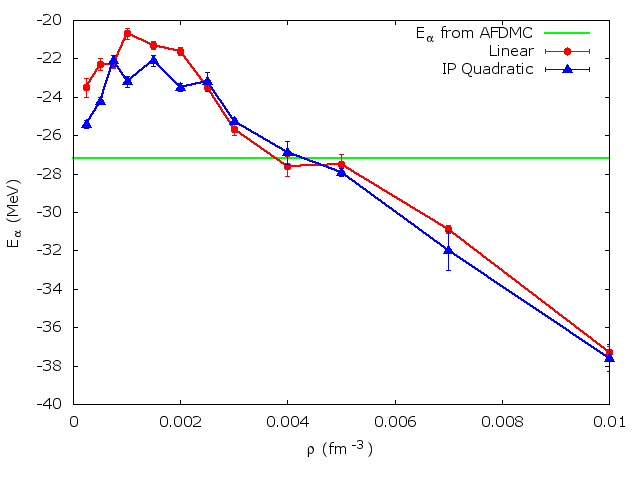
\includegraphics[width=0.7\textwidth]{figures/alpha.png}
   \caption{Energy of 2 protons and 2 neutrons with 12 free neutrons as calculated with Equation~\ref{equ:alphaenergy14n2p} as calculated with linear and quadratic correlations. The green horizontal line indicates the alpha particle energy as calculated with AFDMC using the same AV6$'$ interaction and quadratic correlations.}
   \label{fig:alpha}
\end{figure}
If the free neutrons did not interact with the formed alpha particle it would be expected that the alpha particle energy would agree with previous AFDMC calculations, the results of which are indicated with a green horizontal line. At densities below 0.0025 fm$^{-3}$ the alpha particle is underbound by a few MeV for both linear and quadratic correlations. The quadratic correlations do decrease the alpha energy at low densities. Previously I showed that the quadratic correlations had very little effect on the energy of an alpha particle and so the difference in energy for the linear and quadratic correlations must be related to the alpha-neutron interactions. In addition, the energy for each individual calculation of $\epsilon_\text{14n2p}$ and $\epsilon_\text{14n}$ were decreased with quadratic correlations with respect to linear correlations. The difference between quadratic and linear correlations seems to be the most important for most densities below 0.0025 fm$^{-3}$.

The discrepancy in alpha particle energy at low densities must be due to the excess neutrons deforming the alpha particle. To verify that 2 protons and 2 neutrons, without any free neutrons, will give the correct energy in a periodic box I have calculated the energy of 2 protons and 2 neutrons in various boxes of different densities as shown in Figure~\ref{fig:alpha2n2p}.
\begin{figure}[h!]
   \centering
   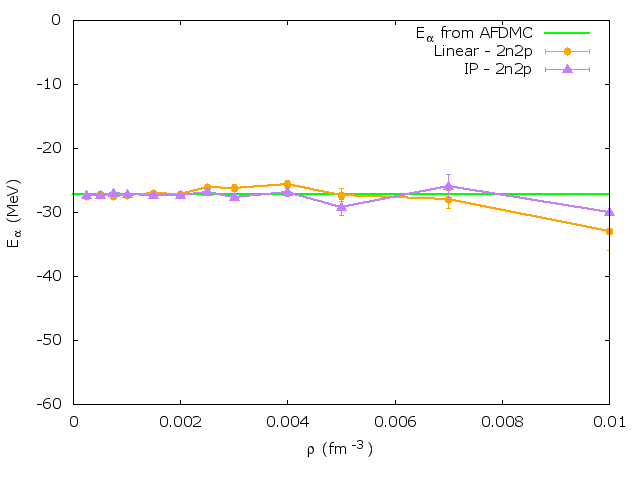
\includegraphics[width=0.7\textwidth]{figures/2n2p.png}
   \caption{Energy of 2 protons and 2 neutrons as calculated with linear and quadratic correlations. The green horizontal line indicates the alpha particle energy as calculated with AFDMC using the same AV6$'$ interaction and quadratic correlations.}
   \label{fig:alpha2n2p}
\end{figure}
The energy at low densities is much closer to the alpha particle energy as calculated with AFDMC.

The other possible explanation for the underbinding of the 4 nucleons at low density is that the alpha particle doesn't form at all. To investigate this I have looked at the pair correlations function
\begin{equation}
   g_\mathcal{O}(r) = \frac{1}{4\pi r^2} \bra{\Psi}\sum\limits_{i<j}\mathcal{O}_{ij}\delta(r-r_{ij})\ket{\Psi},
\end{equation}
where I have specifically looked at the case where the operator is the $pp$ operator. The $g_{pp}(r)$ distribution gives the probability of finding two protons at a distance $r$ from each other. I have plotted these for a few of the densities for which energies were calculated in Figure~\ref{fig:gpp}.
\begin{figure}[h!]
   \centering
   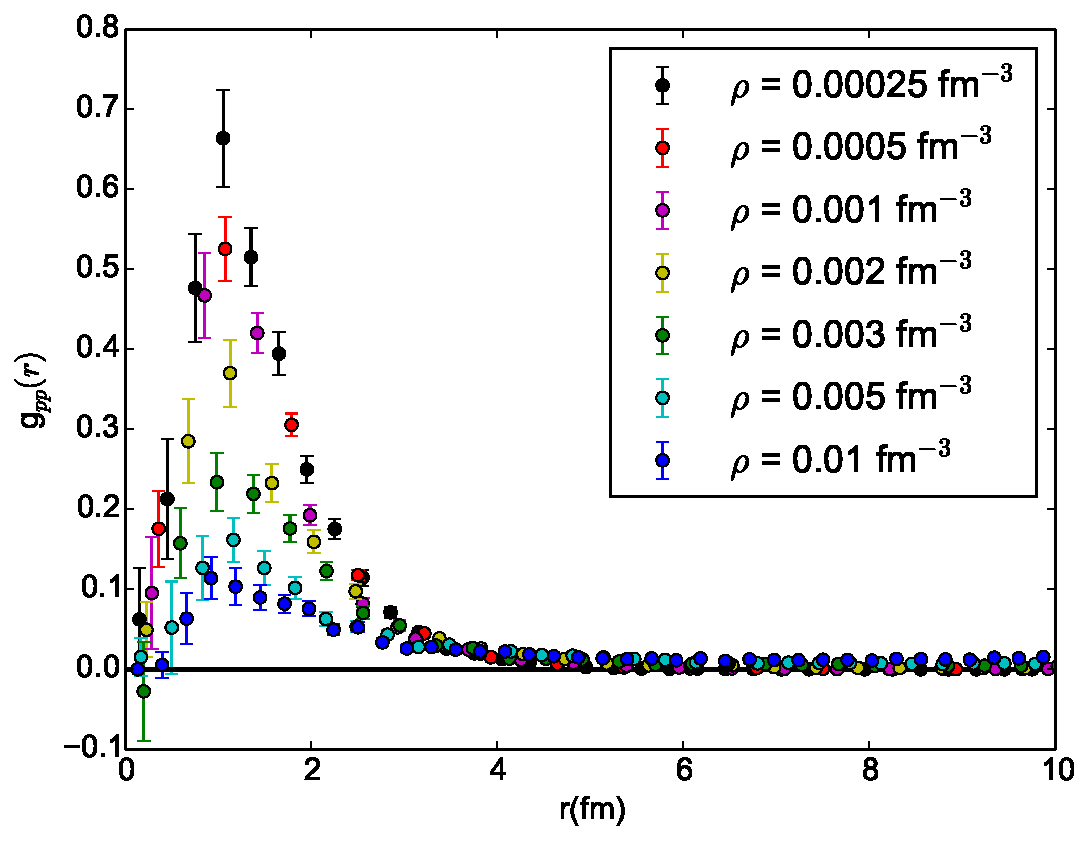
\includegraphics[width=0.7\textwidth]{figures/gpp.pdf}
   \caption{Pair correlations functions, $g_{pp}$ that give the probability of finding 2 protons a distance $r$ from each other. This is only shown for a few of the densities calculated to keep the figure less busy.}
   \label{fig:gpp}
\end{figure}
It is clear to see that as the density decreases the probability of finding the 2 protons at a close distance to each other increases. This is consistent with the formation of an alpha particle. The opposite is true, that as the density increases the protons are more likely to be found separated at larger distances, indicating the dissipation of the alpha particle at high densities. This can be seen in Figure~\ref{fig:gpp_small} which is simply showing more detail to the high separation tail in Figure~\ref{fig:gpp}
\begin{figure}[h!]
   \centering
   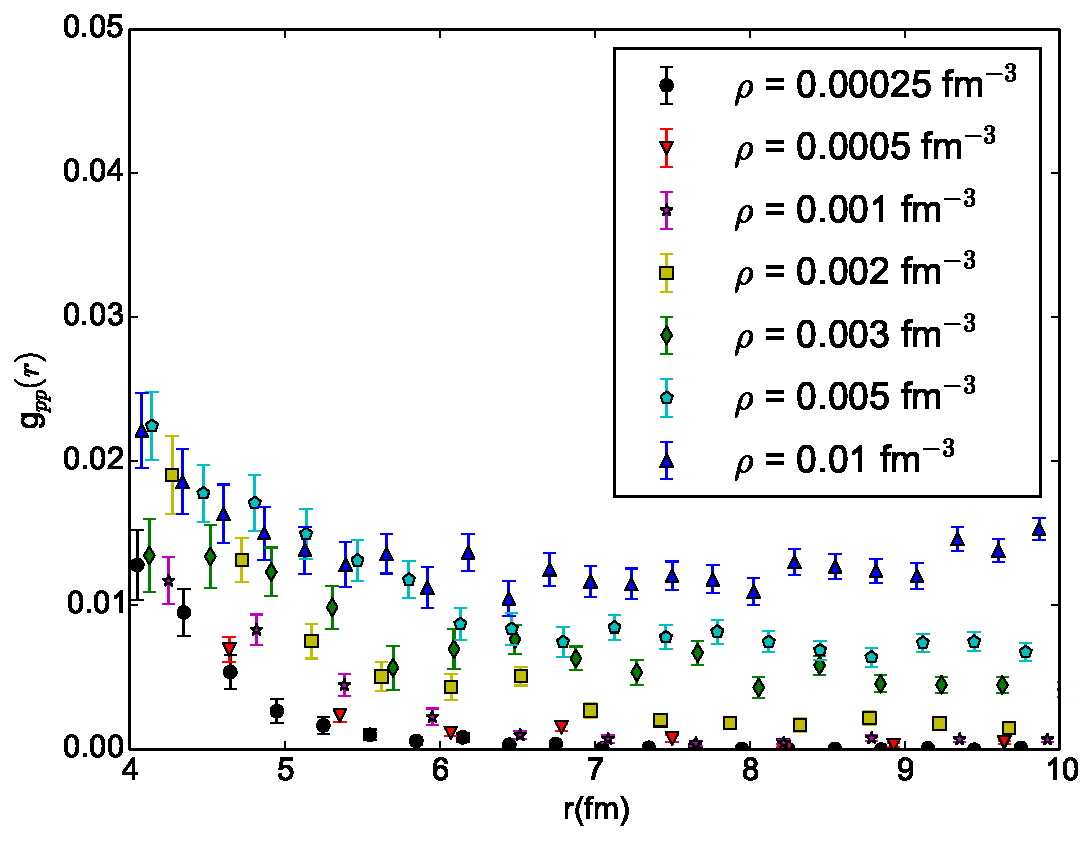
\includegraphics[width=0.7\textwidth]{figures/gpp_small.pdf}
   \caption{Large separation part of the pair correlations functions $g_{pp}$ at different densities.}
   \label{fig:gpp_small}
\end{figure}

This provides good evidence that an alpha particle is forming at low densities. I have also calculated the pair distribution function for the alpha particle as calculated in the continuum, as opposed to the periodic box. In Figure~\ref{fig:gpp_compare} I have plotted this against the $g_{pp}$ pair distribution functions for the 14 neutrons with 2 protons at $\rho=0.00025$ fm$^{-3}$ as calculated with both linear and quadratic correlations. I have increased the resolution of the $g_{pp}$ calculation to show more detail.
\begin{figure}[h!]
   \centering
   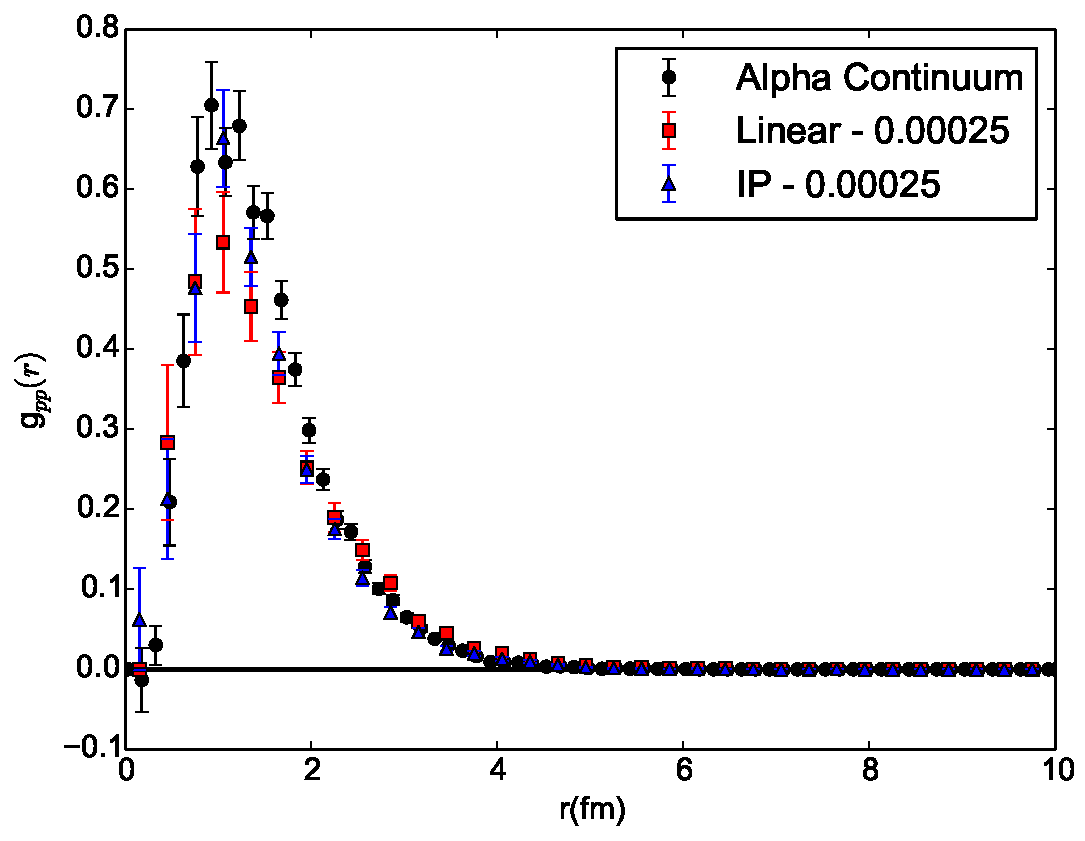
\includegraphics[width=0.7\textwidth]{figures/gpp_compare.pdf}
   \caption{Proton-proton pair distribution functions calculated in the continuum compared to the calculation of 14 neutrons and 2 protons in a periodic box with $\rho=0.00025$ fm$^{-3}$. The $g_{pp}$ calculations in the box have increased resolution compared to those in earlier plots to show more detail. Both linear and IP quadratic correlations were used for the calculations in a box.}
   \label{fig:gpp_compare}
\end{figure}
As was seen before both the linear and IP quadratic correlations seem to be forming an alpha particle, but the IP quadratic correlations provide a better fit to the pair correlation function of the alpha particle as calculated in the continuum, consistent with the energy calculations.

The energy can be split up into the different components of the AV6$'$ potential to study where the binding comes from and where the largest difference in the linear and quadratic correlations occurs. The alpha particle energy as split up into the AV6$'$ components for both linear and IP quadratic correlations is shown in Figure~\ref{fig:av6_alpha}.
\begin{figure}[h!]
   \centering
   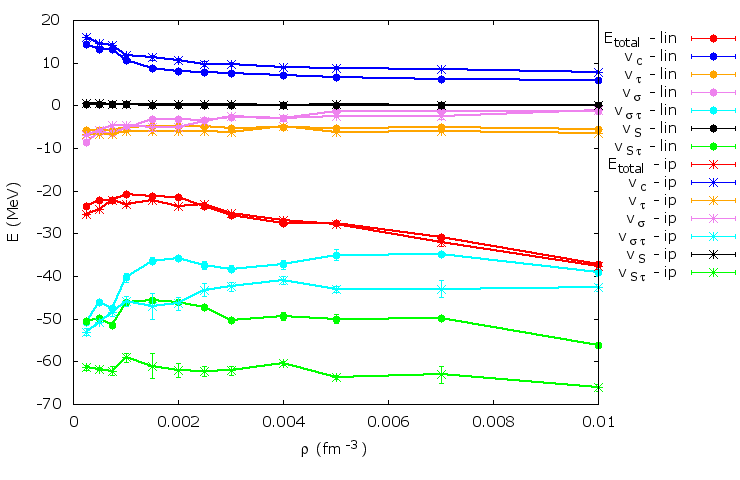
\includegraphics[width=0.9\textwidth]{figures/av6_alpha.png}
   \caption{Alpha particle energy as calculated with Equation~\ref{equ:alphaenergy14n2p} for each piece of the AV6$'$ potential for both linear and IP quadratic correlations.}
   \label{fig:av6_alpha}
\end{figure}
The spin-isospin $\sigma\tau$ and tensor-isospin $S\tau$ operators from one-pion exchange are the operators most effected by the additional correlations in the improved wave function. In addition, the spin-isospin operators is fairly constant at high densities, but decreases for low densities, indicating that it is partially responsible for the alpha particle formation at low densities. This is expected as one-pion exchange is responsible for the long range binding of nuclei.

\section{Conclusion and Outlook}
As mentioned before, one of the most important parts of the calculation is to have a good estimate for the trial wave function that is possible and inexpensive to calculate. So far we have implemented and tested a method for improving the trial wave function used in AFDMC calculation of nuclei and nuclear matter. We have done this by including independent pair and the full quadratic terms in the correlation operator which currently only has linear terms. The addition of these optimized terms has caused the energy of ${}^{4}$He, ${}^{16}$O and SNM to decrease.

Another way to improve the trial wave function is to include more terms in the expansion of the product correlation operator in Eq.~\ref{equ:prodpsi}. As we have learned from the independent pair expansion that we implemented, this would get computationally intractable as the number of particles gets large. Another alternative is to rewrite the correlation operator in terms of a Hubbard-Stratanovich transformation as is done with the spin-isospin dependent part of the propagator in Sec.~\ref{sec:AFDMC}. Future work will be done to handle the correlation operators in this way. We will also be searching for additional ways to improve the trial wave function.

With an improved trial wave function we will be using AFDMC to investigate some interesting aspects of nuclear physics and nuclear astrophysics. For example, we will be investigating the formation of deuteron and alpha particle clusters at various densities in mostly neutron matter. Many types of clustering in physics deal with two particles at a time. Alpha particles are thus a special case of four fermion clustering due to the two additional isospin degrees of freedom in addition to the two spin states for spin 1/2 particles. Work has been done to show the light clustering ($A\leq4$) and condensation of particles in nuclear systems, \cite{schuck2007,schuck2013_1,schuck2013_2} including neutron stars \cite{avancini2010,avancini2012,raduta2014}. We plan to show that the AFDMC method, with an improved nuclear wave function can be used to study properties of light clustering in nuclear systems as well. One way we will be doing this will be to do AFDMC calculation with 14 neutrons in a periodic box with the addition of 2 protons at a variety of densities to observe the formation of an alpha particle in neutron matter. Once these clusters are observed with AFDMC the density can be varied to determine the density at which the clusters dissolve as in Ref.\cite{avancini2012}. This work will be especially applicable to the study of alpha formation in neutron stars.

In conclusion, we have done AFDMC calculations to calculate the energy of ${}^4$He and ${}^{16}$O as well as the energy per particle of SNM. We have done these calculations with both linear correlation terms, linear plus independent pair correlations and linear plus all of the quadratic correlations in the trial wave function. In order to maintain the cluster decomposability of the trail wave function, which is lost with either the linear or independent pair correlations, we will be using the Hubbard-Stratanovich transformation to sample the exponential spin-isospin dependent correlations. This is analogous to the sampling of spin-isospin states in the propagator of AFDMC. We will also be looking for additional ways to improve the trial wave function. We will then be applying these calculations to other interesting nuclear systems such as the clustering of alpha particles in neutron matter.

\newpage
%-----------------------back matter
{\singlespace
% Making the references a "part" rather than a chapter gets it indented at
% level -1 according to the chart: top of page 4 of the document at
% ftp://tug.ctan.org/pub/tex-archive/macros/latex/contrib/tocloft/tocloft.pdf
\addcontentsline{toc}{part}{REFERENCES}
\bibliographystyle{asudis}
%\bibliography{dis}}
\bibliography{../../../../Dropbox/nuclear/papers/references}}
\renewcommand{\chaptername}{APPENDIX}
%\addtocontents{toc}{APPENDIX \par}
\appendix
%\chapter{Raw Data}

\include{vita}
\end{document}
